%%%%%%%%%%%%%%%%%%%%%%%%%%%%%%%%%%%%%%%%%
% Beamer Presentation
% LaTeX Template
% Version 1.0 (10/11/12)
%
% This template has been downloaded from:
% http://www.LaTeXTemplates.com
%
% License:
% CC BY-NC-SA 3.0 (http://creativecommons.org/licenses/by-nc-sa/3.0/)
%
%%%%%%%%%%%%%%%%%%%%%%%%%%%%%%%%%%%%%%%%%

%----------------------------------------------------------------------------------------
%	PACKAGES AND THEMES
%----------------------------------------------------------------------------------------

\documentclass{beamer}

\mode<presentation> {

% The Beamer class comes with a number of default slide themes
% which change the colors and layouts of slides. Below this is a list
% of all the themes, uncomment each in turn to see what they look like.

%\usetheme{default}
%\usetheme{AnnArbor}
%\usetheme{Antibes}
%\usetheme{Bergen}
%\usetheme{Berkeley}
%\usetheme{Berlin}
%\usetheme{Boadilla}
%\usetheme{CambridgeUS}
%\usetheme{Copenhagen}
%\usetheme{Darmstadt}
%\usetheme{Dresden}
%\usetheme{Frankfurt}
%\usetheme{Goettingen}
%\usetheme{Hannover}
%\usetheme{Ilmenau}
%\usetheme{JuanLesPins}
%usetheme{Luebeck}
%\usetheme{Madrid}
%\usetheme{Malmoe}
%\usetheme{Marburg}
%\usetheme{Montpellier}
%\usetheme{PaloAlto}
%\usetheme{Pittsburgh}
%\usetheme{Rochester}
%\usetheme{Singapore}
%\usetheme{Szeged}
%\usetheme{Warsaw}
\usetheme[progressbar=frametitle]{metropolis}

% As well as themes, the Beamer class has a number of color themes
% for any slide theme. Uncomment each of these in turn to see how it
% changes the colors of your current slide theme.

%\usecolortheme{albatross}
%\usecolortheme{beaver}
%\usecolortheme{beetle}
%\usecolortheme{crane}
%\usecolortheme{dolphin}
%\usecolortheme{dove}
%\usecolortheme{fly}
%\usecolortheme{lily}
%\usecolortheme{orchid}
%\usecolortheme{rose}
%\usecolortheme{seagull}
%\usecolortheme{seahorse}
%\usecolortheme{whale}
%\usecolortheme{wolverine}

%\setbeamertemplate{footline} % To remove the footer line in all slides uncomment this line
%\setbeamertemplate{footline}[page number] % To replace the footer line in all slides with a simple slide count uncomment this line

%\setbeamertemplate{navigation symbols}{} % To remove the navigation symbols from the bottom of all slides uncomment this line
}


\usepackage{graphicx} % Allows including images
\usepackage{booktabs} % Allows the use of \toprule, \midrule and \bottomrule in tables
\usepackage[algo2e]{algorithm2e}
%\usepackage{enumitem}
%\usepackage{algorithm}
\usepackage{hyperref}
\usepackage{natbib}
\usepackage{multicol}
\usepackage[utf8]{inputenc}
%\usepackage{graphicx}
%\usepackage{xcolor}
%\usepackage{indentfirst}
\usepackage{amsmath,amsfonts,amsthm}
\usepackage{caption} %for captionof
\usepackage{subcaption}
%\usepackage{booktabs} % Allows the use of \toprule, \midrule and \bottomrule in tables
% Package and patches to include mathematical expressions
%\usepackage{pdflscape}
%\usepackage{chngpage}% allows for temporary adjustment of side margins
%\usepackage{multicol}
\usepackage{tabu}
\usepackage{tikz}
\usetikzlibrary{arrows.meta, calc, fit, tikzmark}
%----------------------------------------------------------------------------------------
%	TITLE PAGE
%----------------------------------------------------------------------------------------

\title[PRS project]{Improve Health Equality for Polygenic Risk Score (PRS) by Joint Penalized Regression of GWAS Summary Statistics from Two Ancestries} % The short title appears at the bottom of every slide, the full title is only on the title page

\author [PL] { \\ \vspace{0.5cm} \\Peng Liu} % Your name
\institute[Merck]{%\includegraphics[width=1.1cm]{school_logo.png} \\\ 
\\Biostatistics \& Research Decision Sciences\\ Merck Research Laboratories}

\date{\today} % Date, can be changed to a custom date

\begin{document}

\begin{frame}
\titlepage % Print the title page as the first slide
\end{frame}

%----------------------------------------------
% Background
%-----------------------------------------------
%\section{Background}
%\begin{frame}
%\frametitle{High-throughput technologies} 
%\begin{figure}[b]
%\includegraphics[width=12cm, height=8cm]{images/Microarray_NGS.png}
%\centering
%\end{figure}
% insert a picture about next generation sequencing
%\end{frame}

%\begin{frame}{Analysis of High dimensional omics data}
%    \begin{figure}[b]
%\includegraphics[width=10cm, height=8cm]{images/overview1.png} % update this image
%\centering
%\end{figure}
%\end{frame}

%\begin{frame}{Analysis of High dimensional omics data}
%    \begin{figure}[b]
%\includegraphics[width=10cm, height=8cm]{images/overview2.png} % update this image
%\centering
%\end{figure}
%\end{frame}

\begin{frame}{Genetic Disorders}
\begin{itemize}
    \item Mendelian disorders are caused by specific mutations in single gene. e.g. cystic fibrosis
    \item Complex genetic disorders result from combined effect of tens to hundreds of gene mutations each with a small effect. 
\end{itemize}

\begin{figure}[h]	\noindent\makebox[\textwidth]{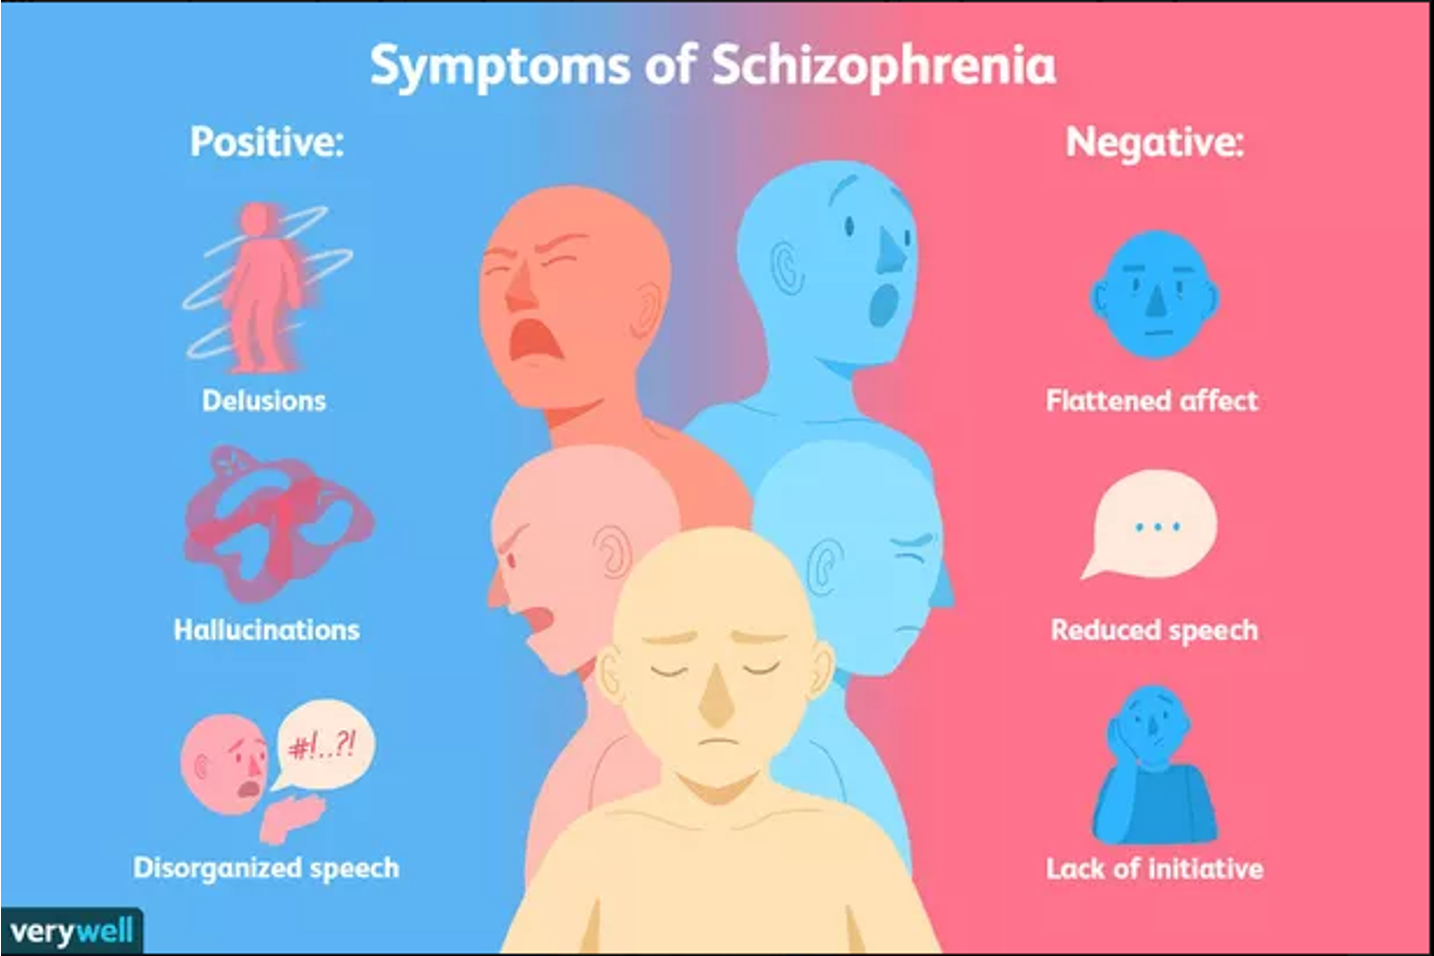
\includegraphics[scale=0.25]{images/Schizophrenia.png}}
    \caption{Schizophrenia}
    \label{fig:Schizophrenia}
        {\tiny https://www.verywellmind.com/}
\end{figure}
\end{frame}

\begin{frame}{Genome-Wide Association Studies (GWAS)}

\begin{figure}
\centering
\begin{subfigure}{.5\textwidth}
  \centering
  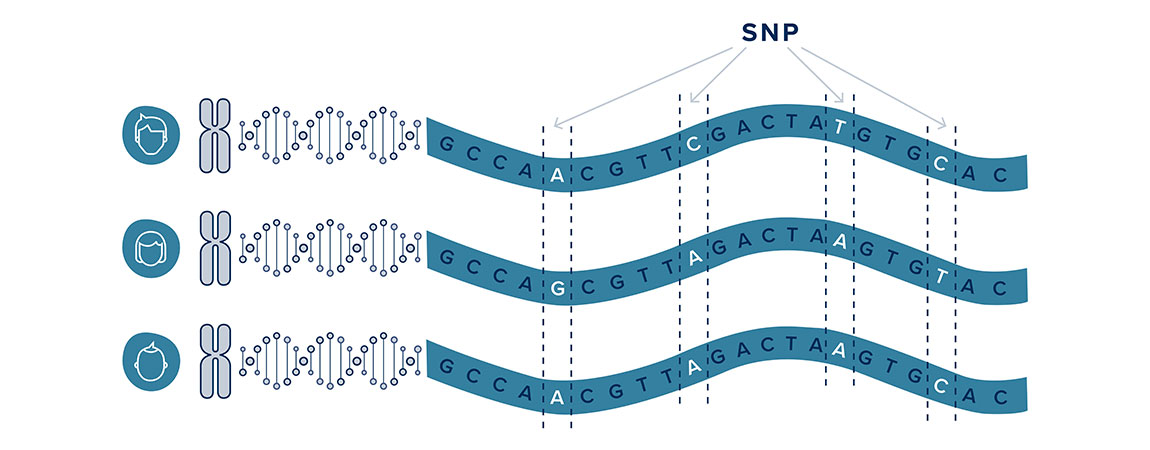
\includegraphics[width=.9\linewidth]{images/SNP.jpeg}
  \caption{Single Nucleotide Polymorphism (SNP)}
  \label{fig:distribution}
              %{\tiny Lewis \& Vassos (2020) Genome Med.}
\end{subfigure}%
\begin{subfigure}{.5\textwidth}
  \centering
  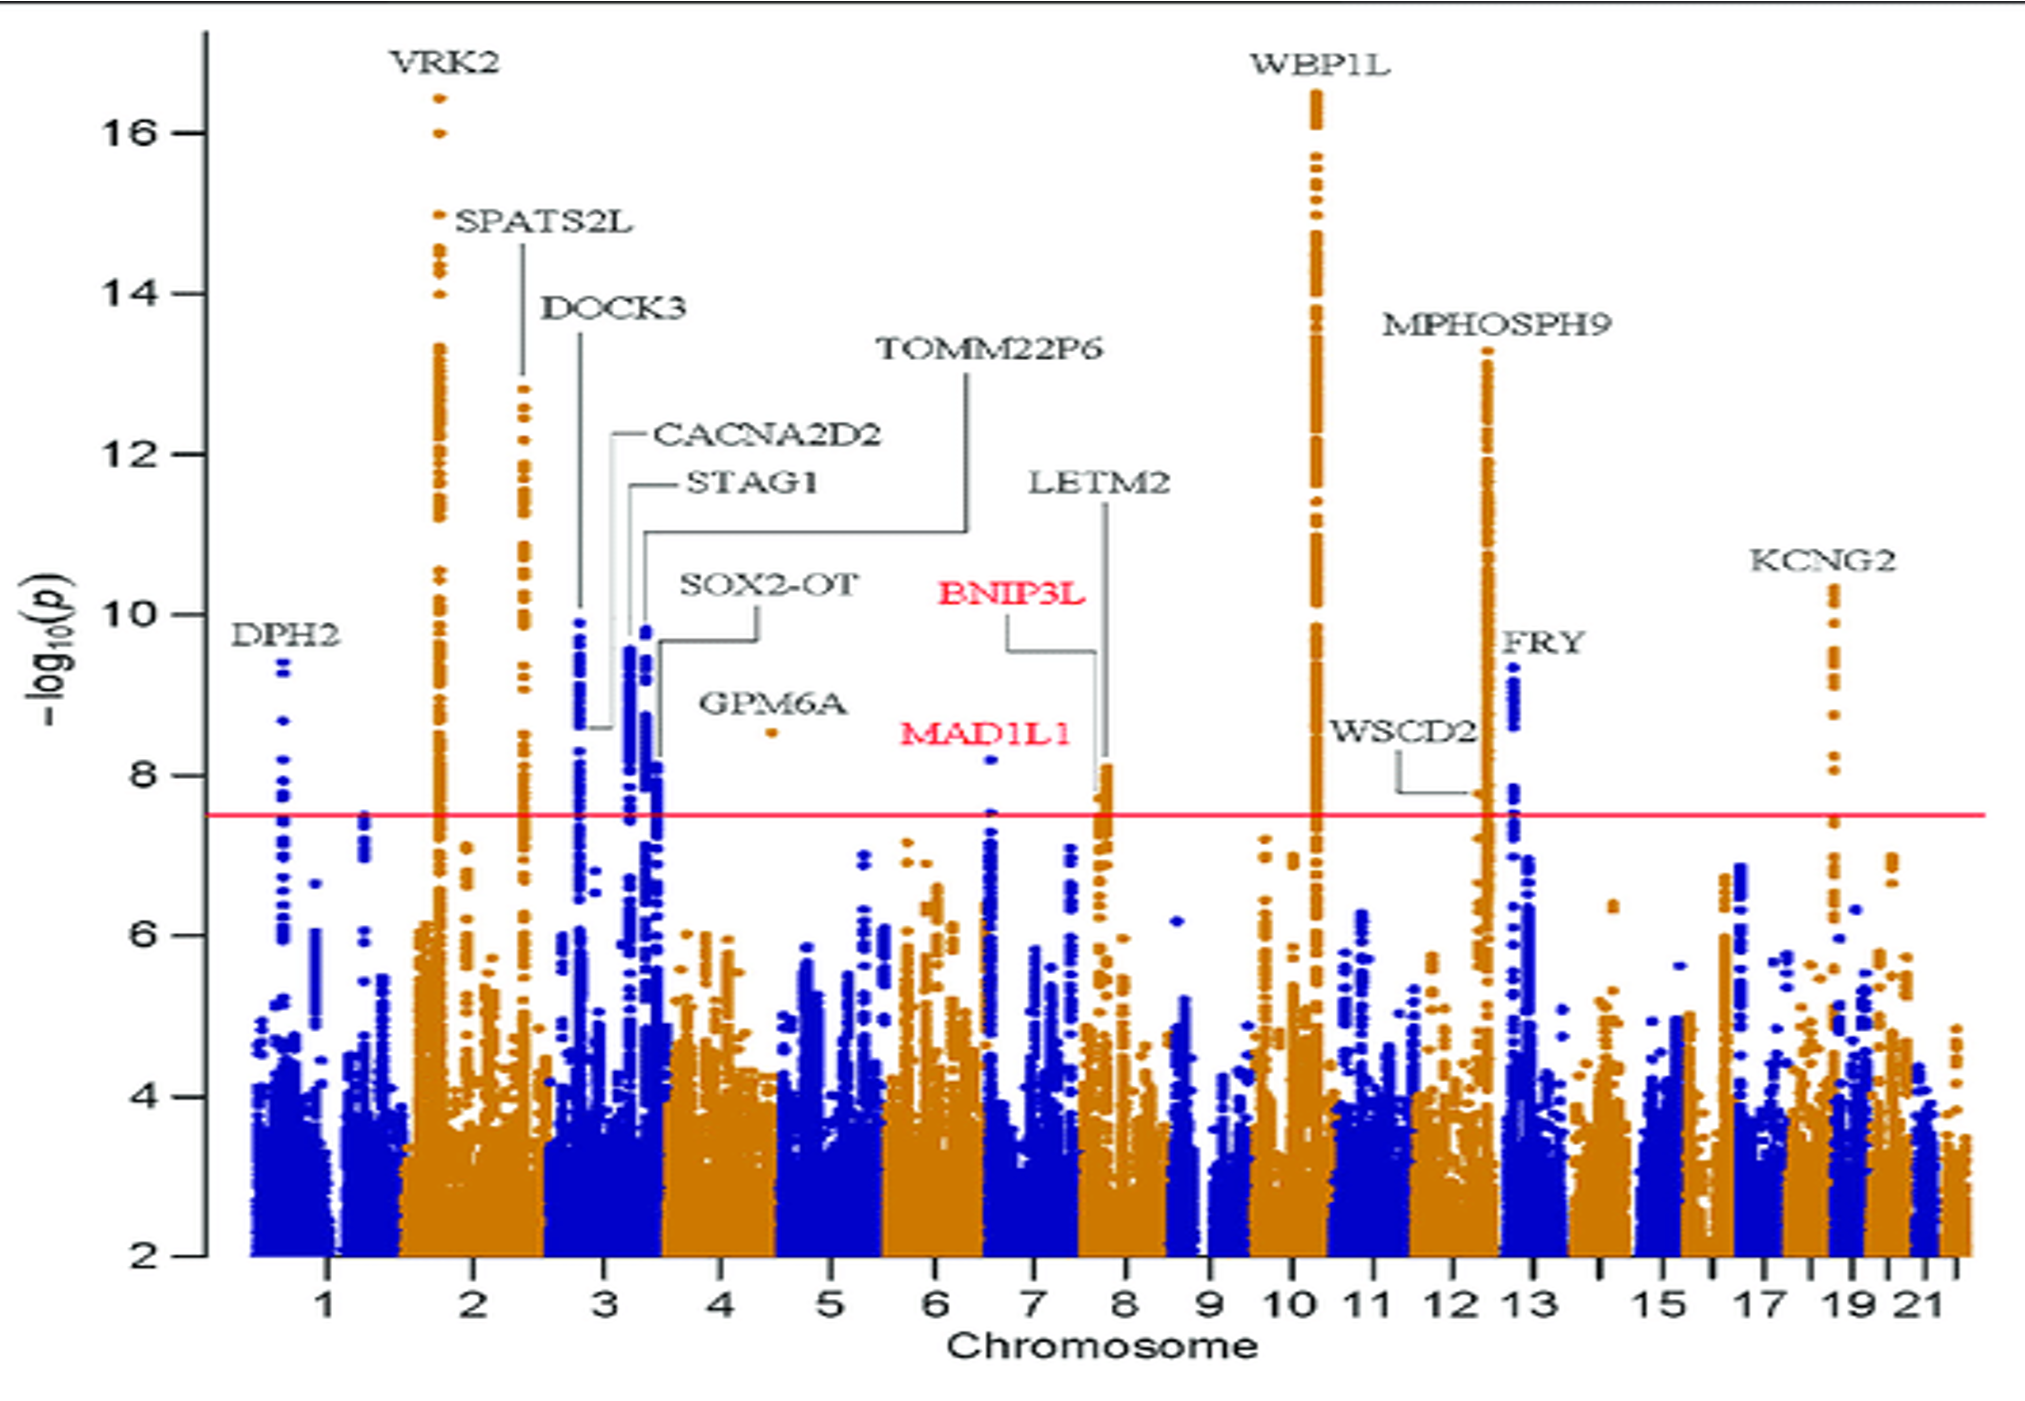
\includegraphics[width=.9\linewidth]{images/GWAS_SCZ.png}
    \caption{Manhattan plot for genome-wide association studies (GWAS)}
    \label{fig:GWAS Schizophrenia}
\end{subfigure}
%\caption{A figure with two subfigures}
\label{fig:GWAS}
\end{figure}

%\begin{itemize}
    %\item Advances in technology now enable us to perform large-scale DNA sequencing.
    %\item It is possible to combine the information from hundreds or thousands of genetic variants to estimate disease risk at the individual level
\begin{itemize}
    %\item GWAS routinely includes tens of thousands of subjects, but most studies are conducted on people of European ancestry
    \item The genetic risk is most often assessed through the polygenic risk score (PRS), a weighted sum of a number of risk alleles. 
\end{itemize}

%\end{itemize}

\end{frame}

\begin{frame}{Weighting up the Risks}
%\begin{itemize}

A polygenic score (PGS) or polygenic risk score (PRS) is a weighted sum of the risk alleles

\begin{equation}
    PRS_i=\sum_{j}\beta_j x_{ij}
\end{equation}

\begin{figure}
\centering
\begin{subfigure}{.5\textwidth}
  \centering
  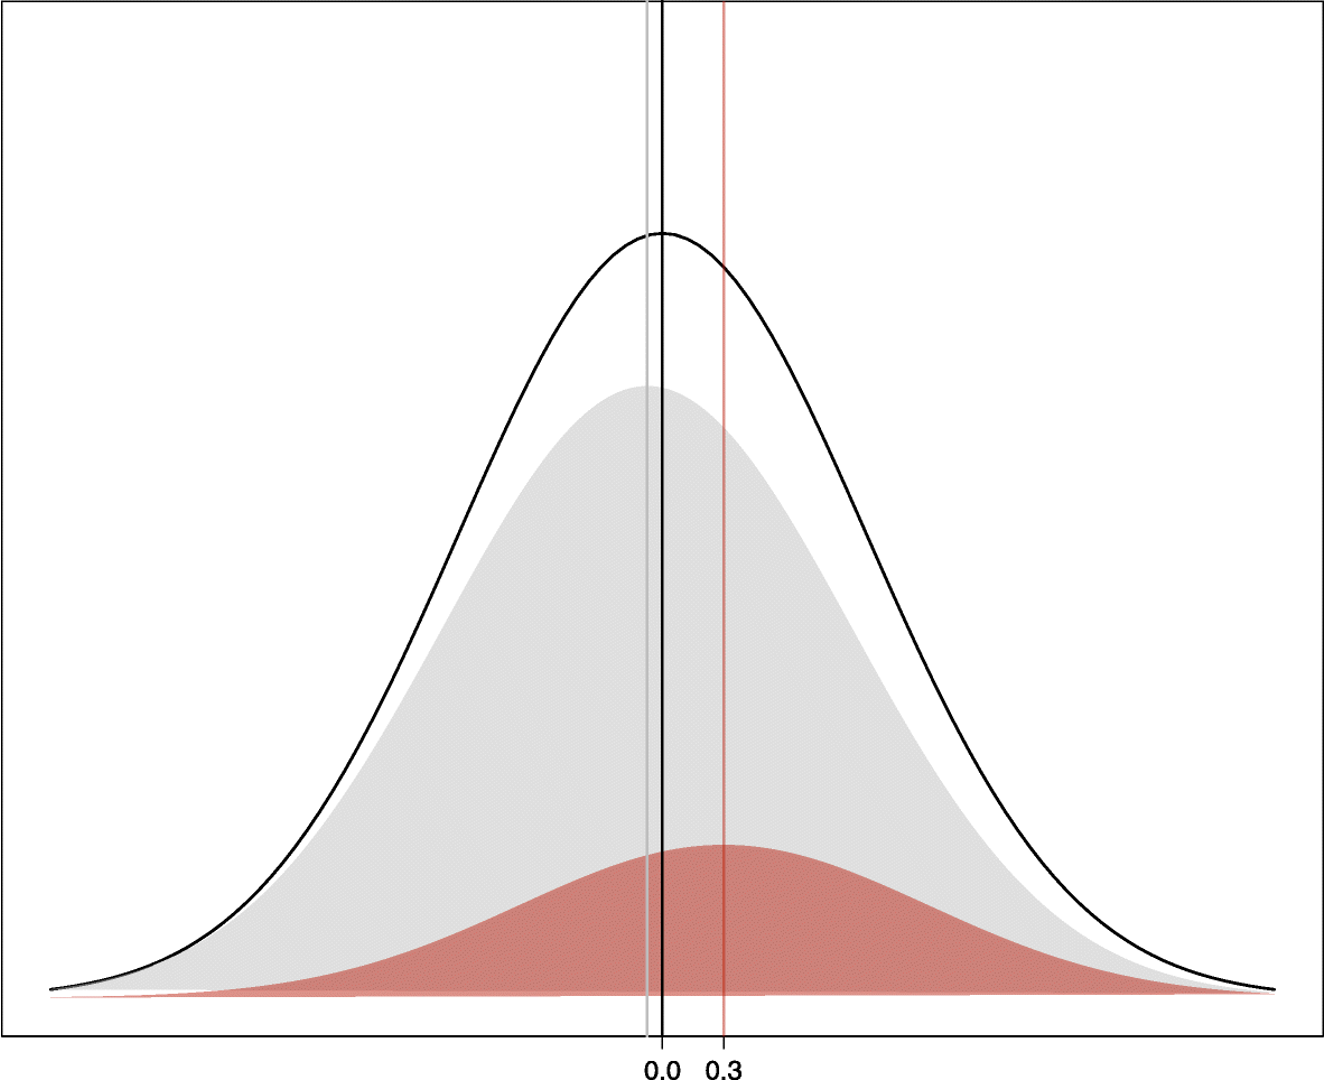
\includegraphics[width=.7\linewidth]{images/PRS_distribution.png}
  \caption{Distribution of PRS}
  \label{fig:distribution}
              {\tiny Lewis \& Vassos (2020) Genome Med.}
\end{subfigure}%
\begin{subfigure}{.5\textwidth}
  \centering
  
\includegraphics[width=.7\linewidth]{images/Genotype.png}
  \caption{Genotype matrix}
  \label{fig:genotype}
\end{subfigure}
%\caption{A figure with two subfigures}
\label{fig:}
\end{figure}

%\begin{figure}[h]	\noindent\makebox[\textwidth]{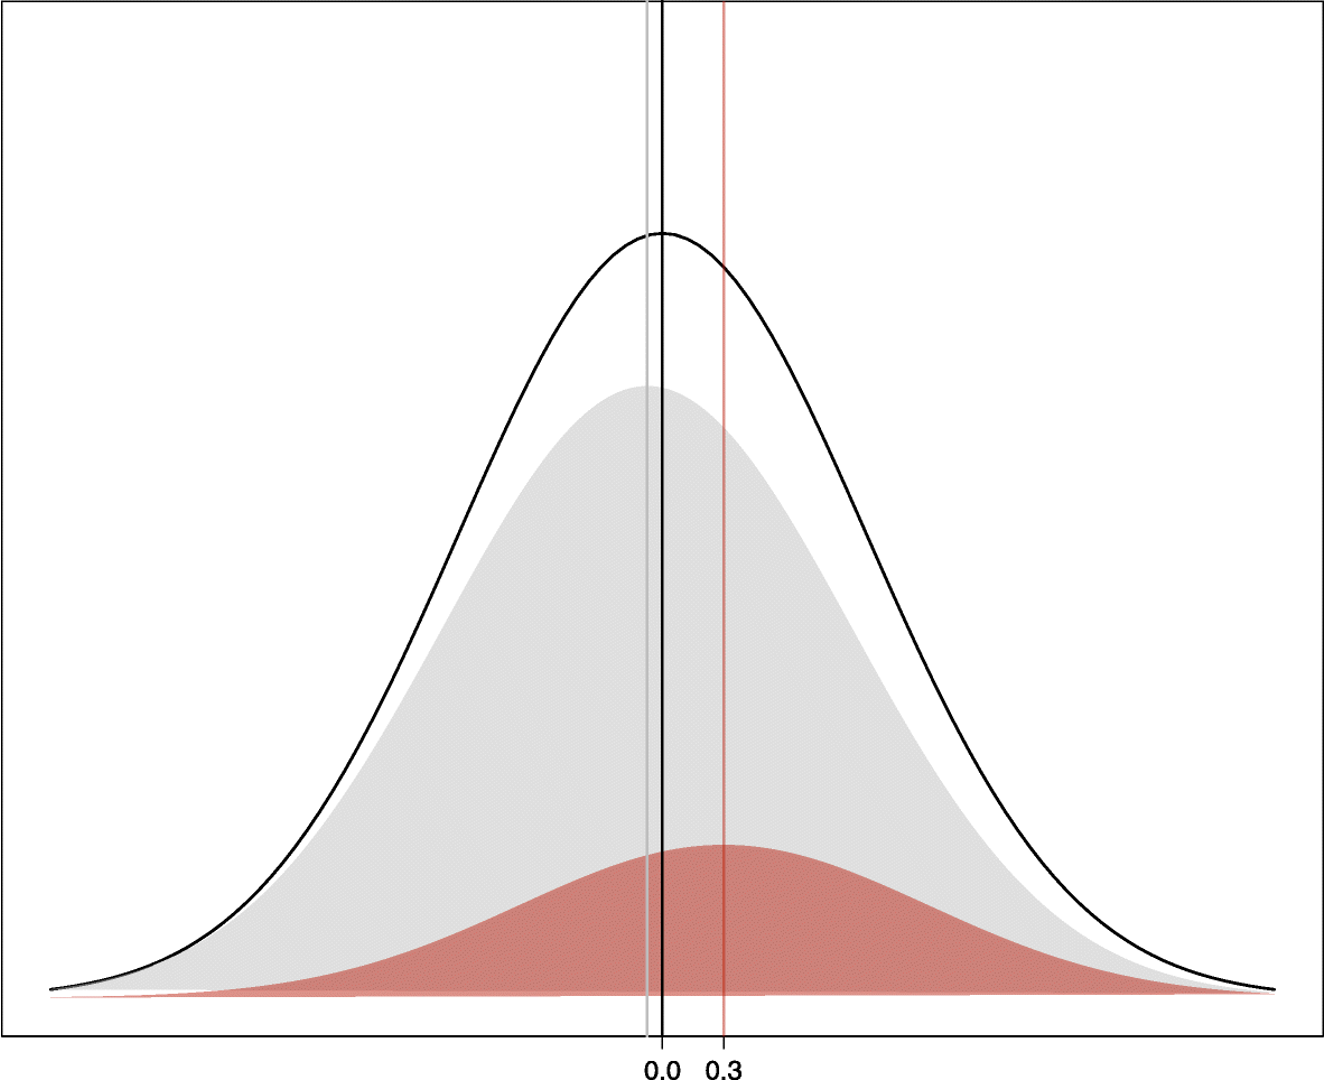
\includegraphics[scale=0.2]{images/PRS_distribution.png}}
%    \caption{Distribution of PRS}
%    \label{fig:distribution}
%            {\tiny Lewis \& Vassos (2020) Genome Med.}
%\end{figure}
    
\end{frame}
%-------------------------------
\begin{frame}{Polygenic Risk Score (PRS)}
In the current PGS Catalog, 2163 polygenic scores over 527 traits have been developed. (This is only part of the whole picture!)
    \begin{figure}[h]	\noindent\makebox[\textwidth]{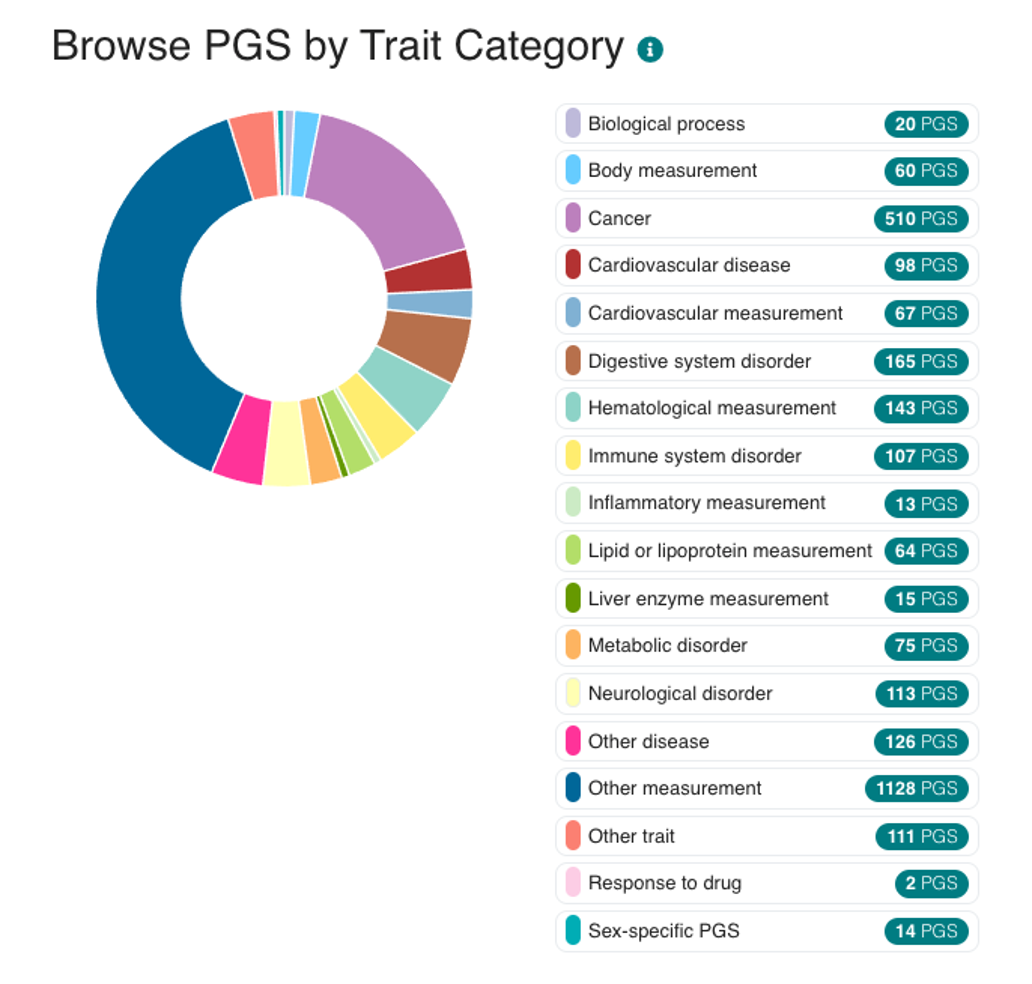
\includegraphics[scale=0.4]{images/PRSTraits.png}}
    \caption{Clinical translation}
    \label{fig:traits}
\end{figure}
\end{frame}

%--------------------------------
\begin{frame}{Polygenic Risk Score (PRS)}
The scores were shown to have potential for broad-scale clinical use
\begin{figure}[h]	\noindent\makebox[\textwidth]{\includegraphics[scale=0.3]{images/clinical_translation.png}}
    \caption{Clinical translation}
    \label{fig:translation}
\end{figure}

\end{frame}

\begin{frame}{Key Issues for PRS Calculation}
\begin{itemize}
\item Selection of SNPs to be included in PRS derivation. 
\item Estimation of $\beta$s
\item Incorporating the correlation of SNPs called Linkage disequilibrium (LD). 
\end{itemize}

%\begin{figure}[h]	\noindent\makebox[\textwidth]{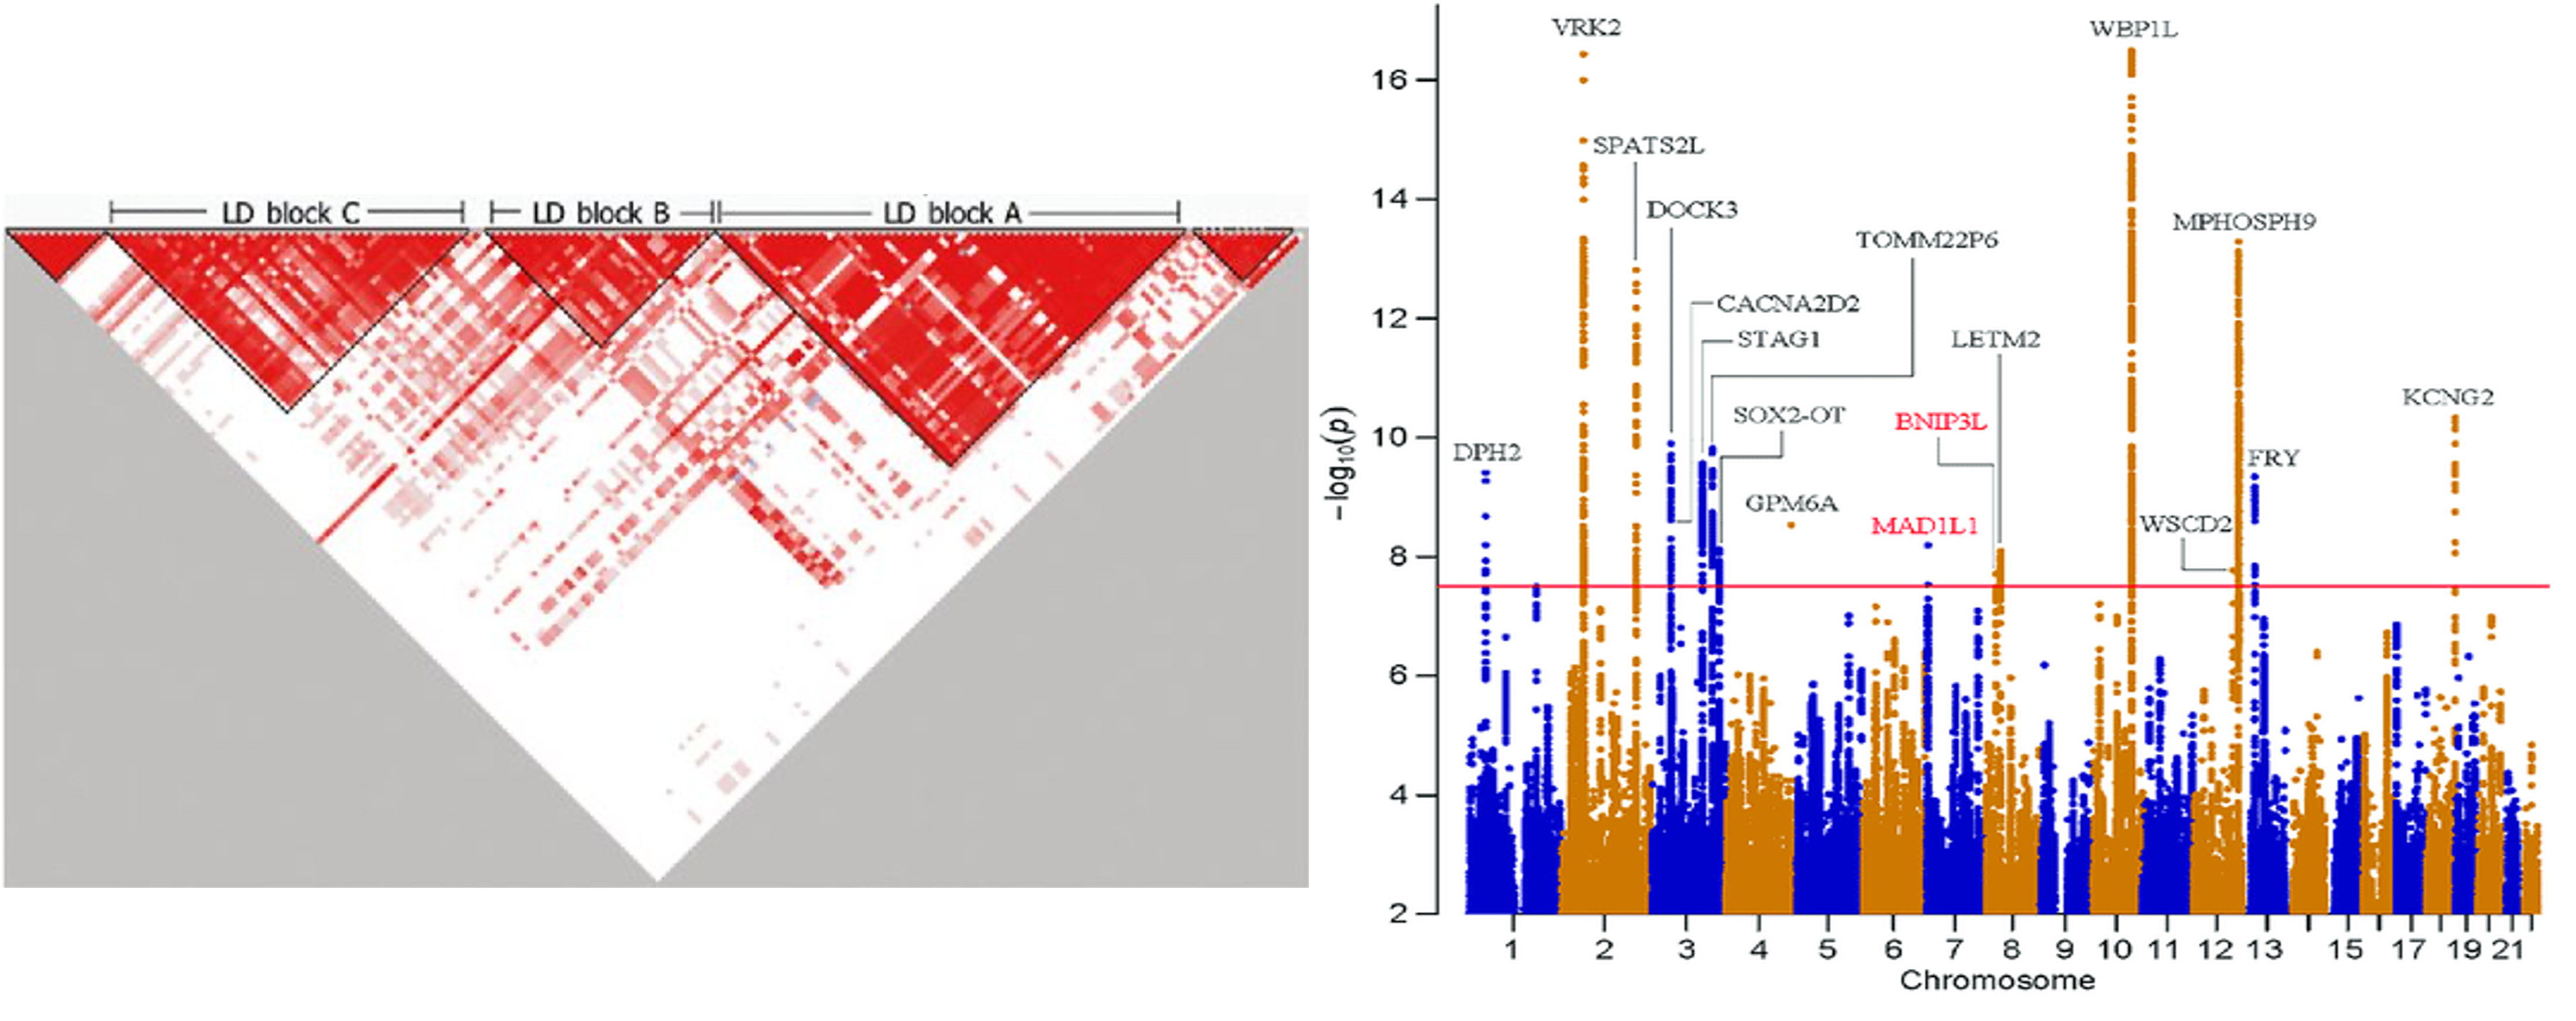
\includegraphics[scale=0.3]{images/LD.png}}
    %\caption{Manhattan plot for the GWAS meta analysis for Schizophrenia and bipolar disorders in East Asian populations}
%    \label{fig:GWAS Schizophrenia}
%\end{figure}

\begin{figure}
\centering
\begin{subfigure}{.5\textwidth}
  \centering
  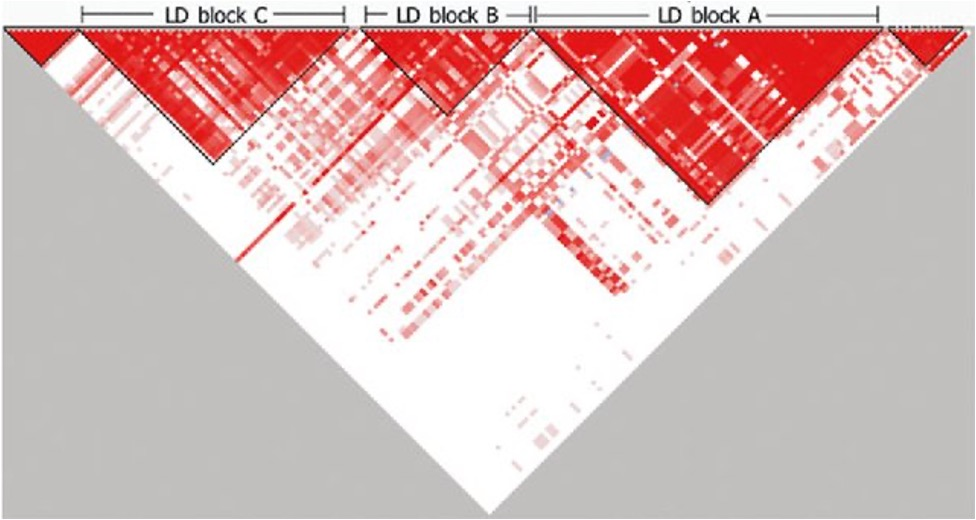
\includegraphics[width=.8\linewidth]{images/LD.jpg}
  \caption{LD blocks of SNPs}
  \label{fig:distribution}
\end{subfigure}%
\begin{subfigure}{.5\textwidth}
  \centering
  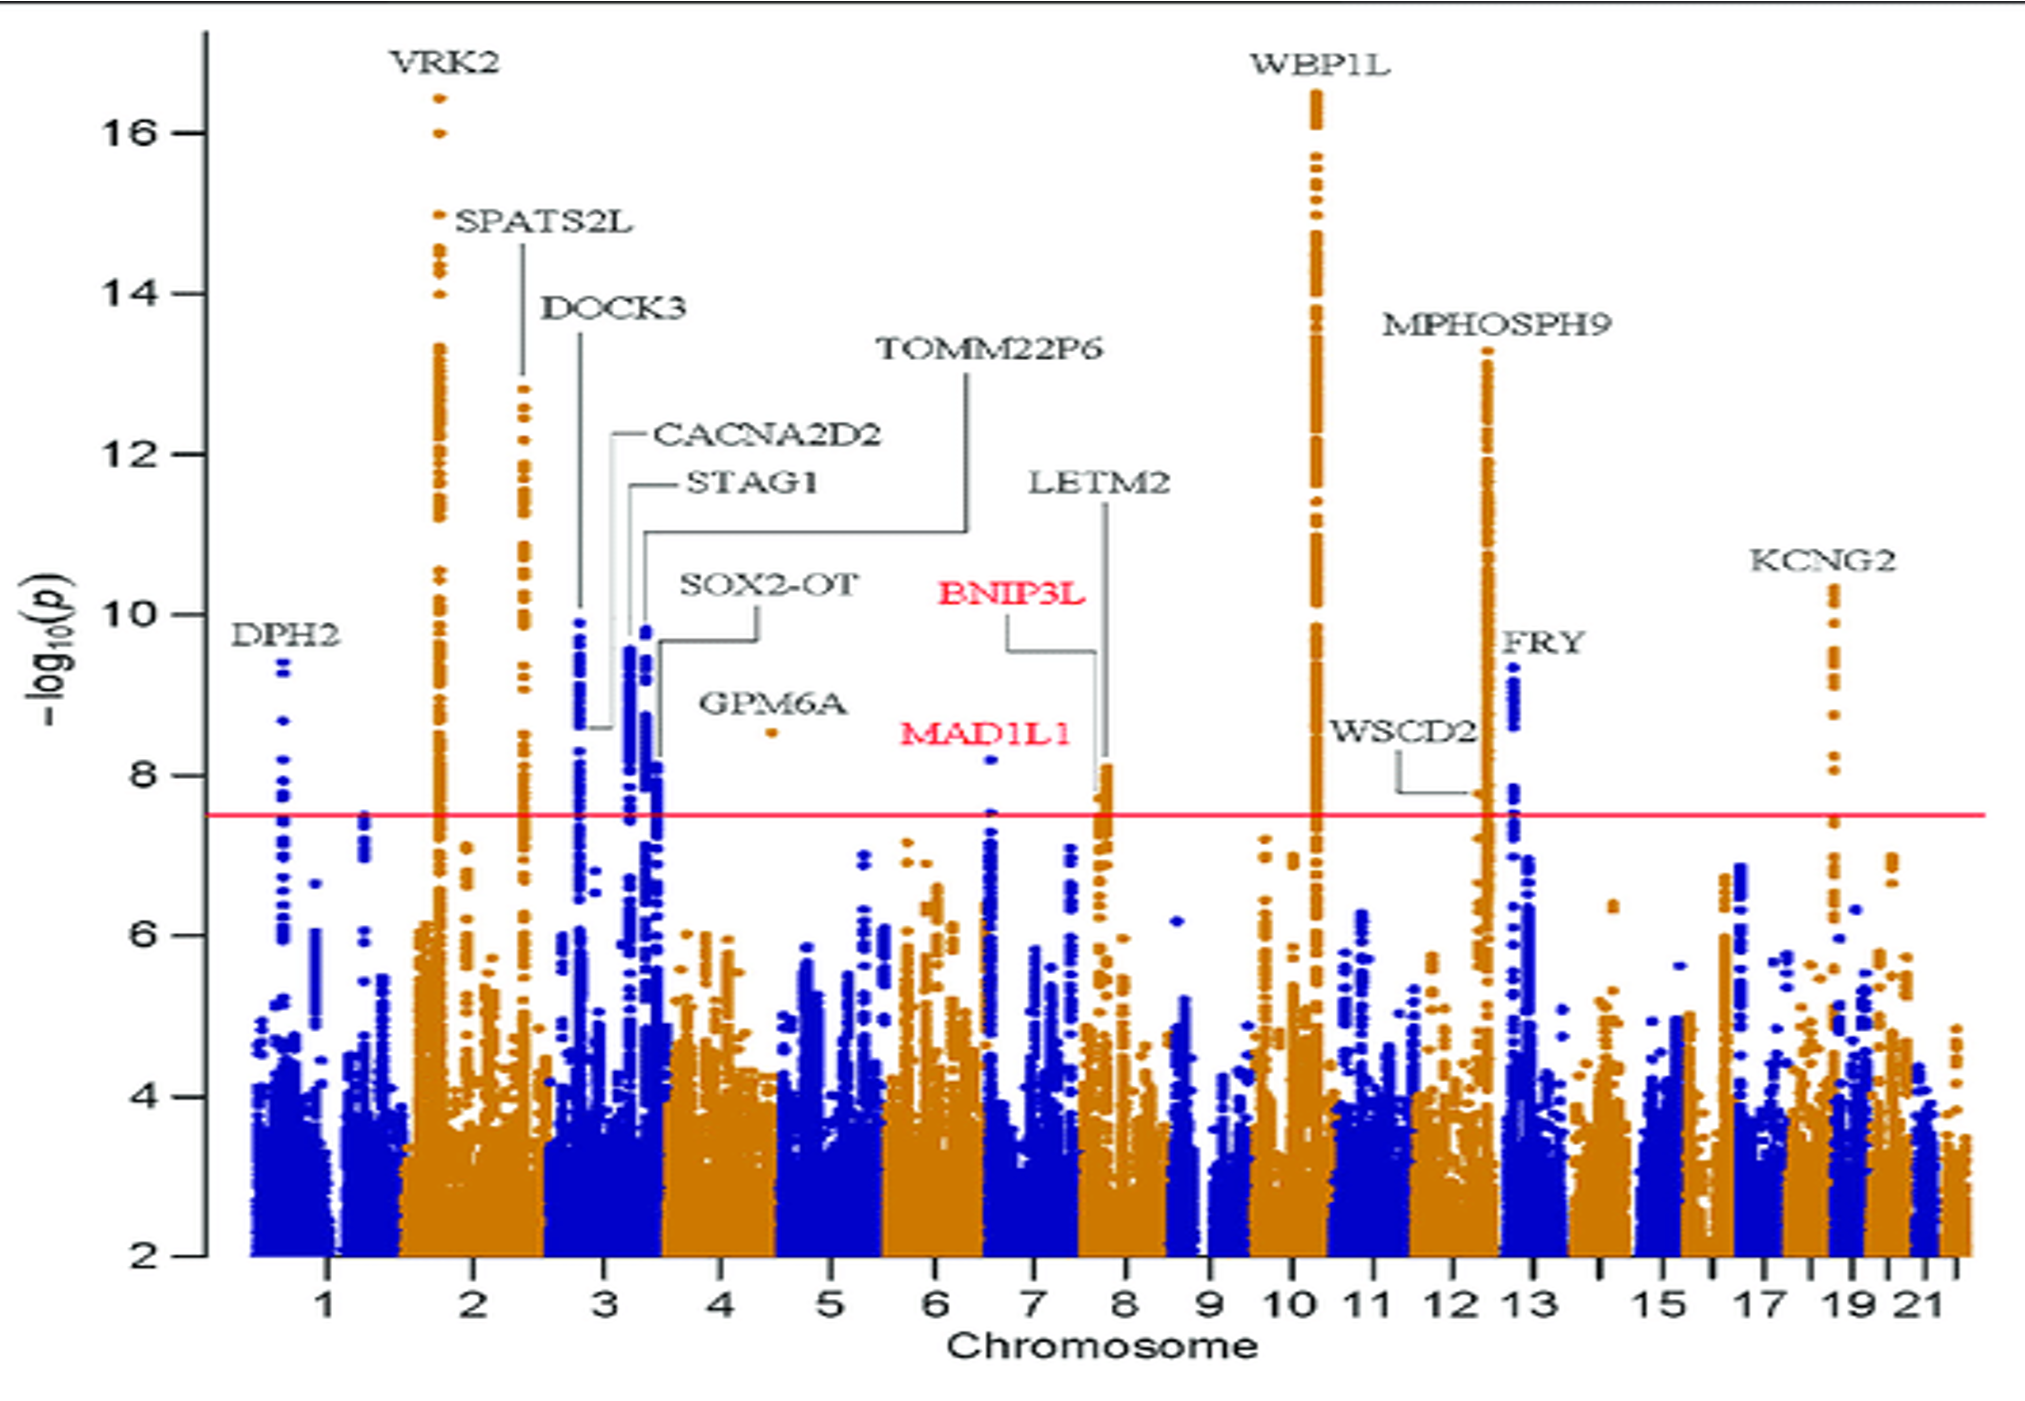
\includegraphics[width=.8\linewidth]{images/GWAS_SCZ.png}
  \caption{GWAS results}
  \label{fig:GWAS}
\end{subfigure}
%\caption{A figure with two subfigures}
\label{fig:}
\end{figure}


\end{frame}

\begin{frame}{Statistical Methods for PRS Derivation}
\begin{itemize}
    \item Pruning and thresholding (P+T)
    \item Frequentest approaches: lassosum
    \item Bayesian approaches: LDpred2, SbayesR
\end{itemize}

%\begin{figure}[h]	\noindent\makebox[\textwidth]{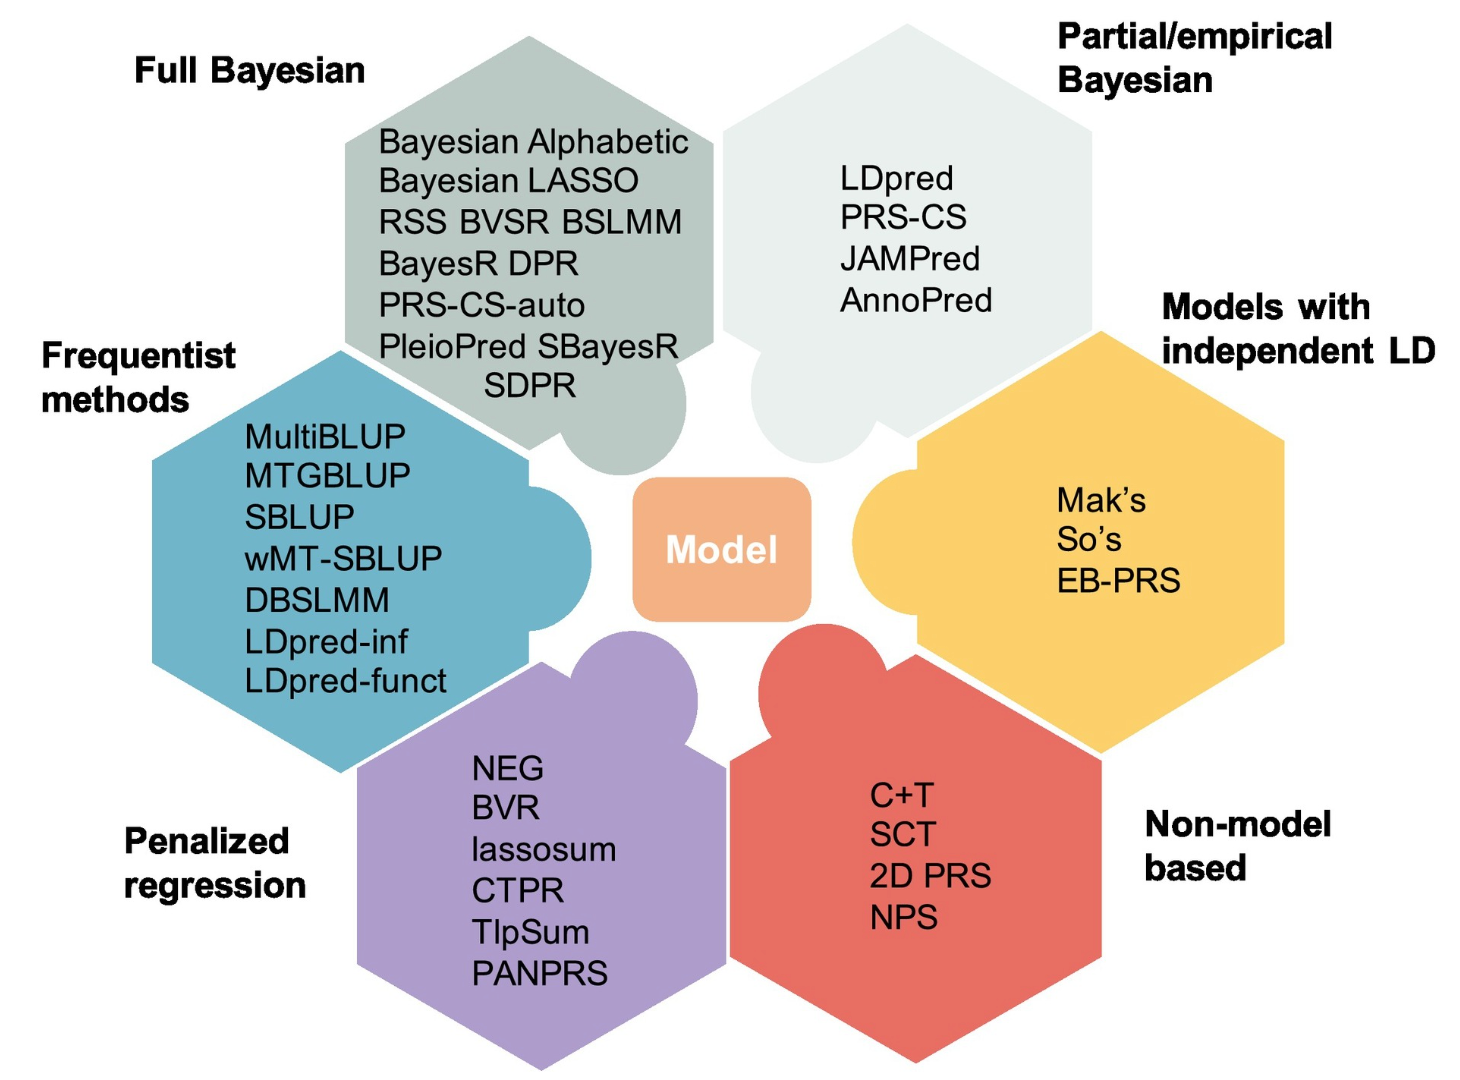
\includegraphics[scale=0.3]{images/Models.png}}
    %\caption{Models}
%    \label{fig:models}
%\end{figure}

\end{frame}

\begin{frame}{Motivation}

\begin{figure}[h]	\noindent\makebox[\textwidth]{
\includegraphics[scale=0.3]{images/Disparities.png}}
    %\caption{Manhattan plot for the GWAS meta analysis for Schizophrenia and bipolar disorders in East Asian populations}
    \label{fig:Disparities}
\end{figure}

%    \begin{enumerate}
        Heath disparities of PRS
        \begin{itemize}
            \item The scores are largely been calculated from European population
            \item Clinical uses of PRS today would systematically afford greater improvement for European-descent populations.
        \end{itemize}
%    \end{enumerate}



\end{frame}

\begin{frame}{Health Disparities of PRS}

The scores are largely been calculated from European population.
    \begin{figure}[h]	\noindent\makebox[\textwidth]{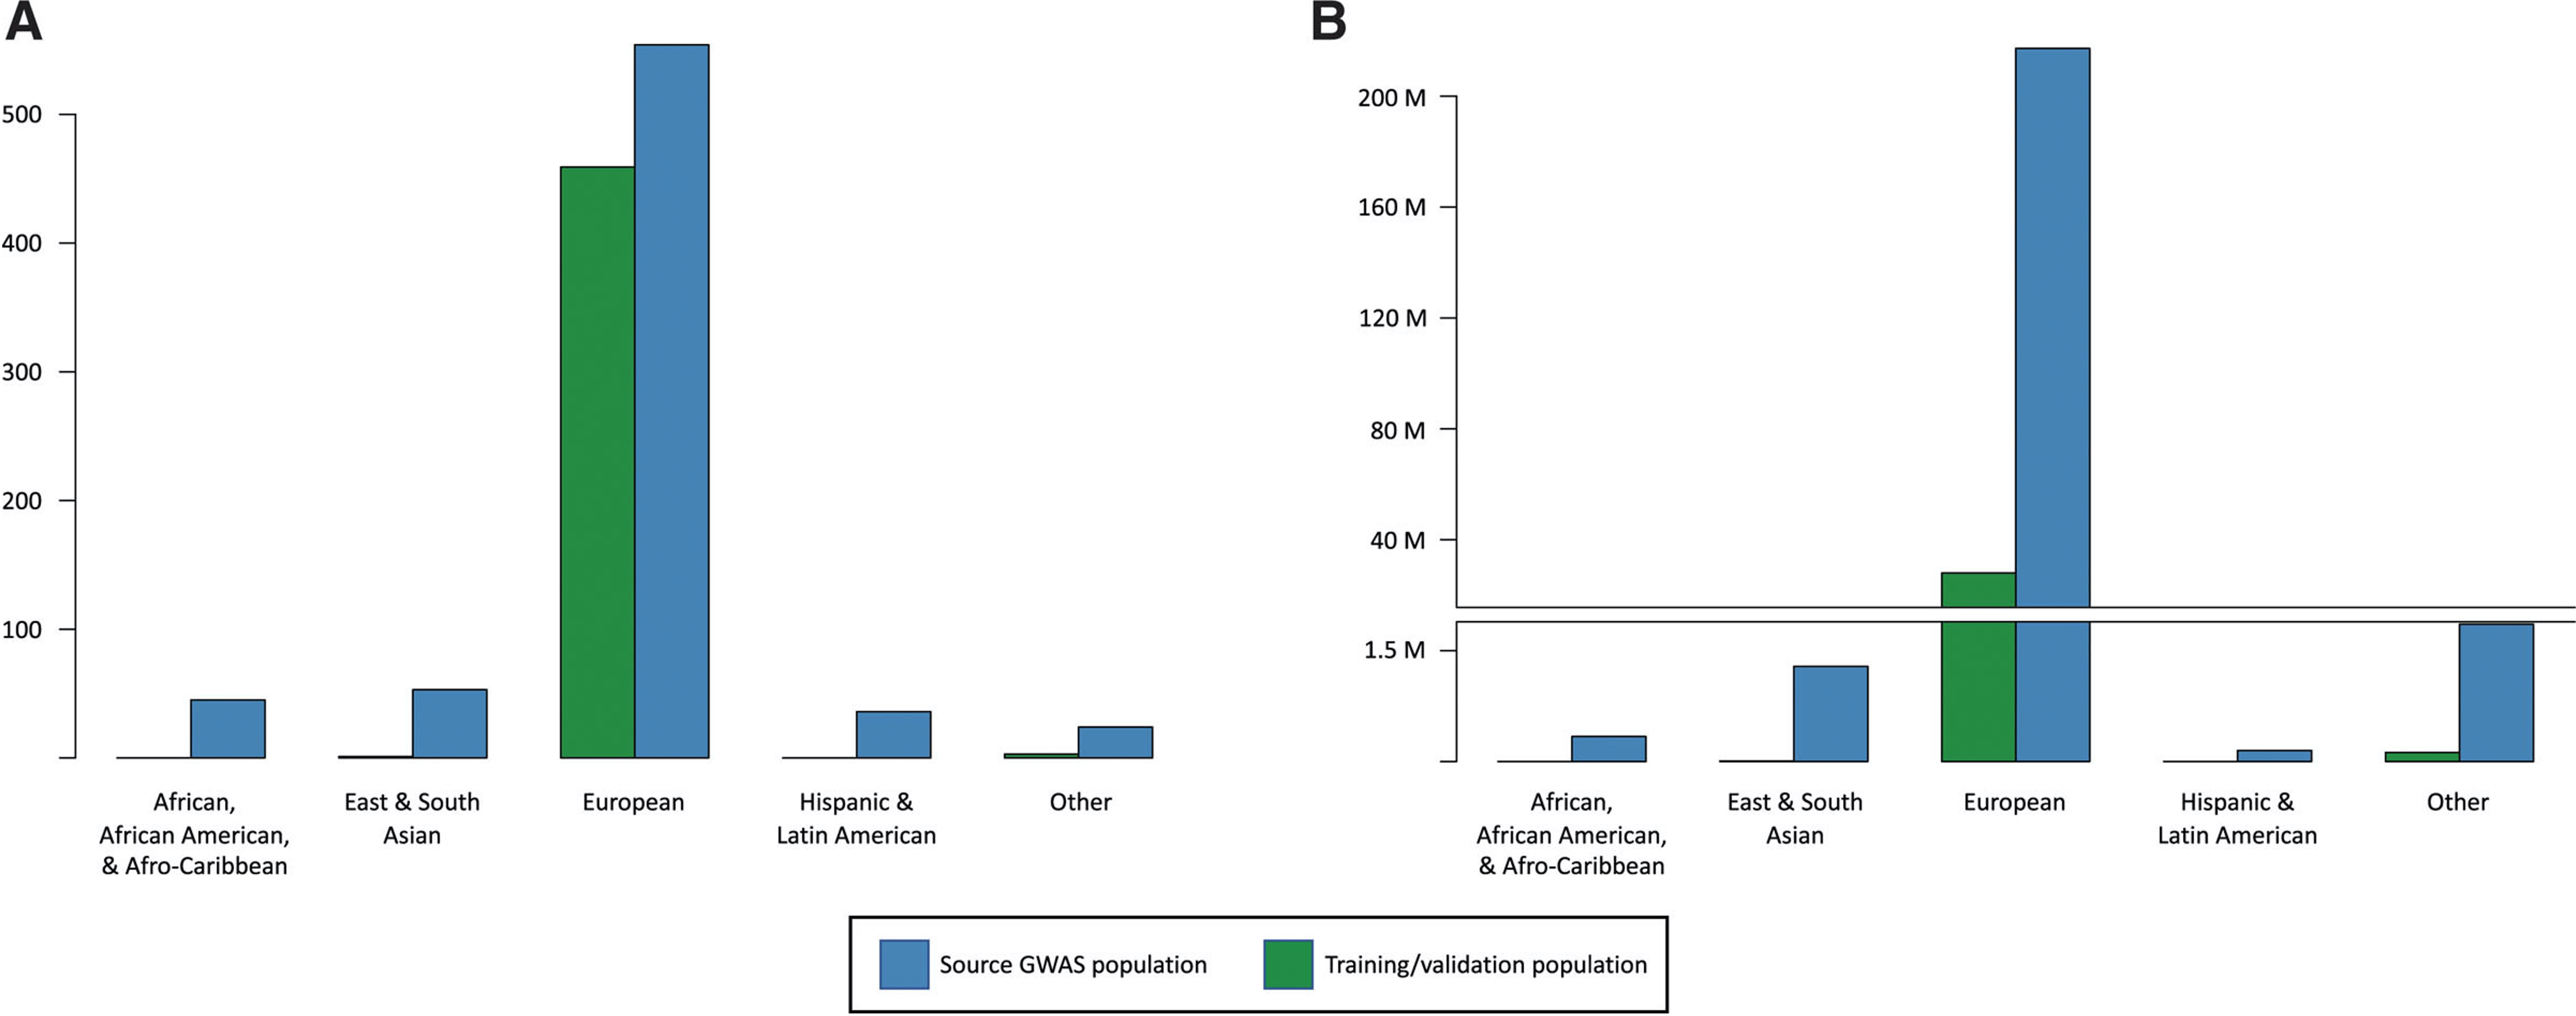
\includegraphics[scale=0.035]{images/PRSPopulations.jpg}}
     {\tiny Clarke et al. (2021) CIRC-GENOM}
    %\caption{Models}
    \label{fig:models}
\end{figure}



\end{frame}

\begin{frame}{Challenges in PRS Portability}

Clinical use of PRS could exacerbate race-based health disparities
\begin{figure}[h]	\noindent\makebox[\textwidth]{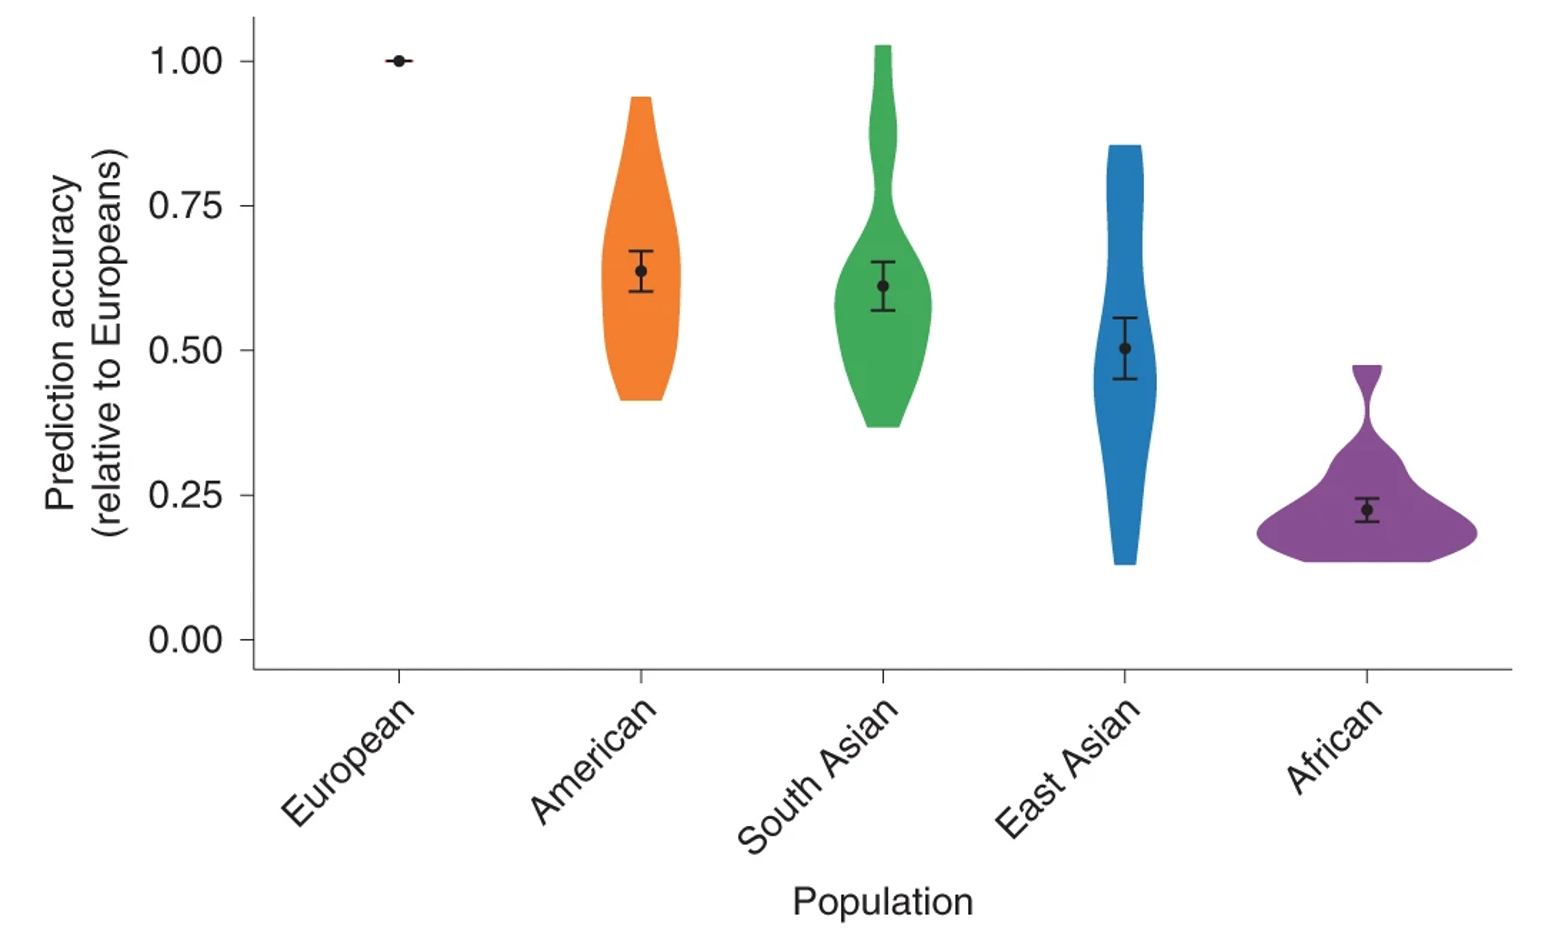
\includegraphics[scale=0.35]{images/Portability.png}}
    %\caption{Models}
         {\tiny Martin et al. (2019) Nature Genetics}
\label{fig:models}
\end{figure}
\end{frame}

\begin{frame}{Possible Explanations}

\begin{itemize}
    \item The causal SNPs of the phenotype might differ, or the risk alleles may have different effect on disease risks across ancestries
    \item The methods do not select causal SNPs, but the SNPs in LD with causal variant. 
\end{itemize}

\begin{figure}[h]	\noindent\makebox[\textwidth]{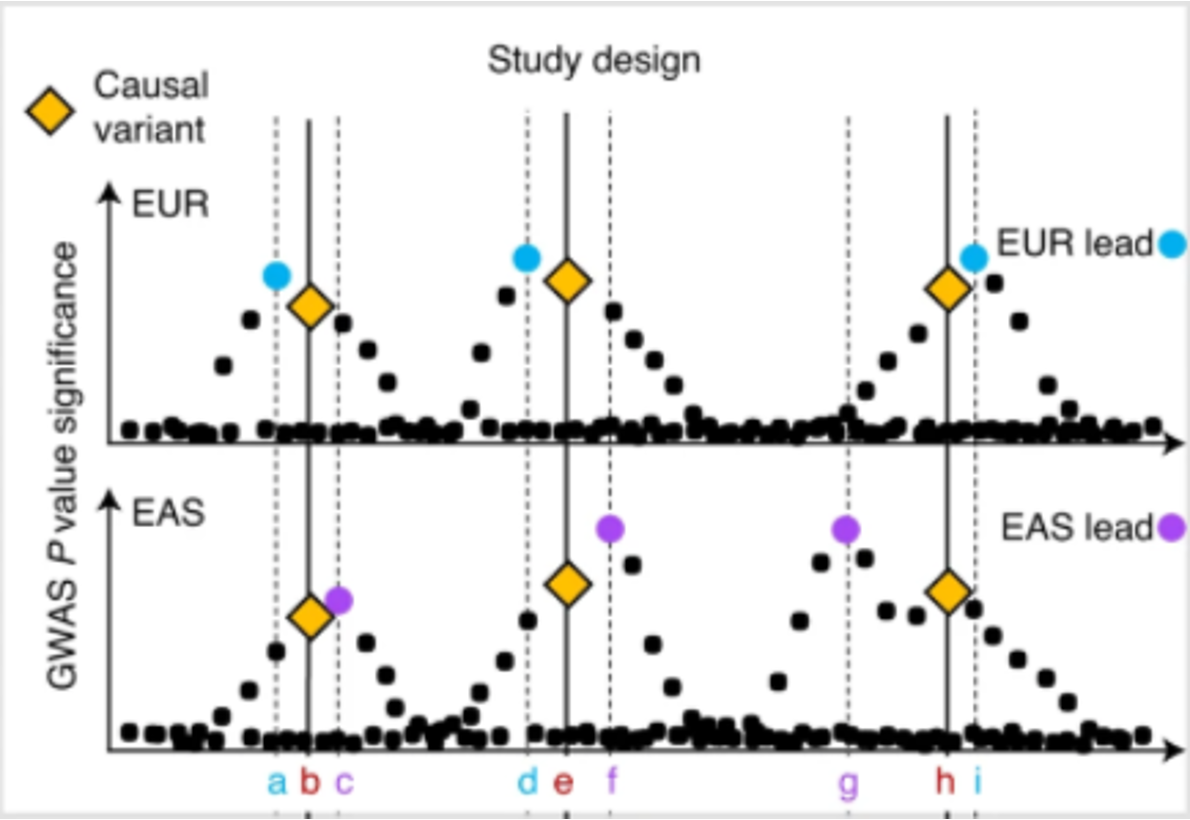
\includegraphics[scale=0.3]{images/LD_EURvsAFR.png}}
    %\caption{LD structure of Europeans(blue) vs African(black)}
    \label{fig:LD}
            {\tiny Amariuta et al. (2020) Nature Genetics}
\end{figure}
    
\end{frame}

%\begin{frame}{What can we do?}
%    Conduct global projects that aim to characterize genomics variation in diverse populations
%    \begin{itemize}
%        \item Neuropsychiatric Genetics in African Populations (NeuroGap)
%        \item All of us: building a large-scale biomedical data resource that reflects the diversity of the US population
%    \end{itemize}
%\end{frame}

\begin{frame}{Sharpening the Scores}

%\begin{enumerate}
    %\item Aim to identify causal SNPs by incorporating functional annotation information
    %\begin{itemize}
    %    \item AnnoPred
    %    \item LDpred-funct
    %\end{itemize}
    %\pause
%Combine genetic information of multiple ancestries.
    \begin{itemize}
        \item PRS can work whether or not the causal SNPs are the same (if LD blocks are similar)
        \item PRS does not work if the LD blocks of the training data are much longer than those for the target population.
        \item Attenuate disparities by incorporating the genetic information from less represented population.
    \end{itemize}
    
%\end{enumerate}

\begin{figure}
\centering
\begin{subfigure}{.5\textwidth}
  \centering
  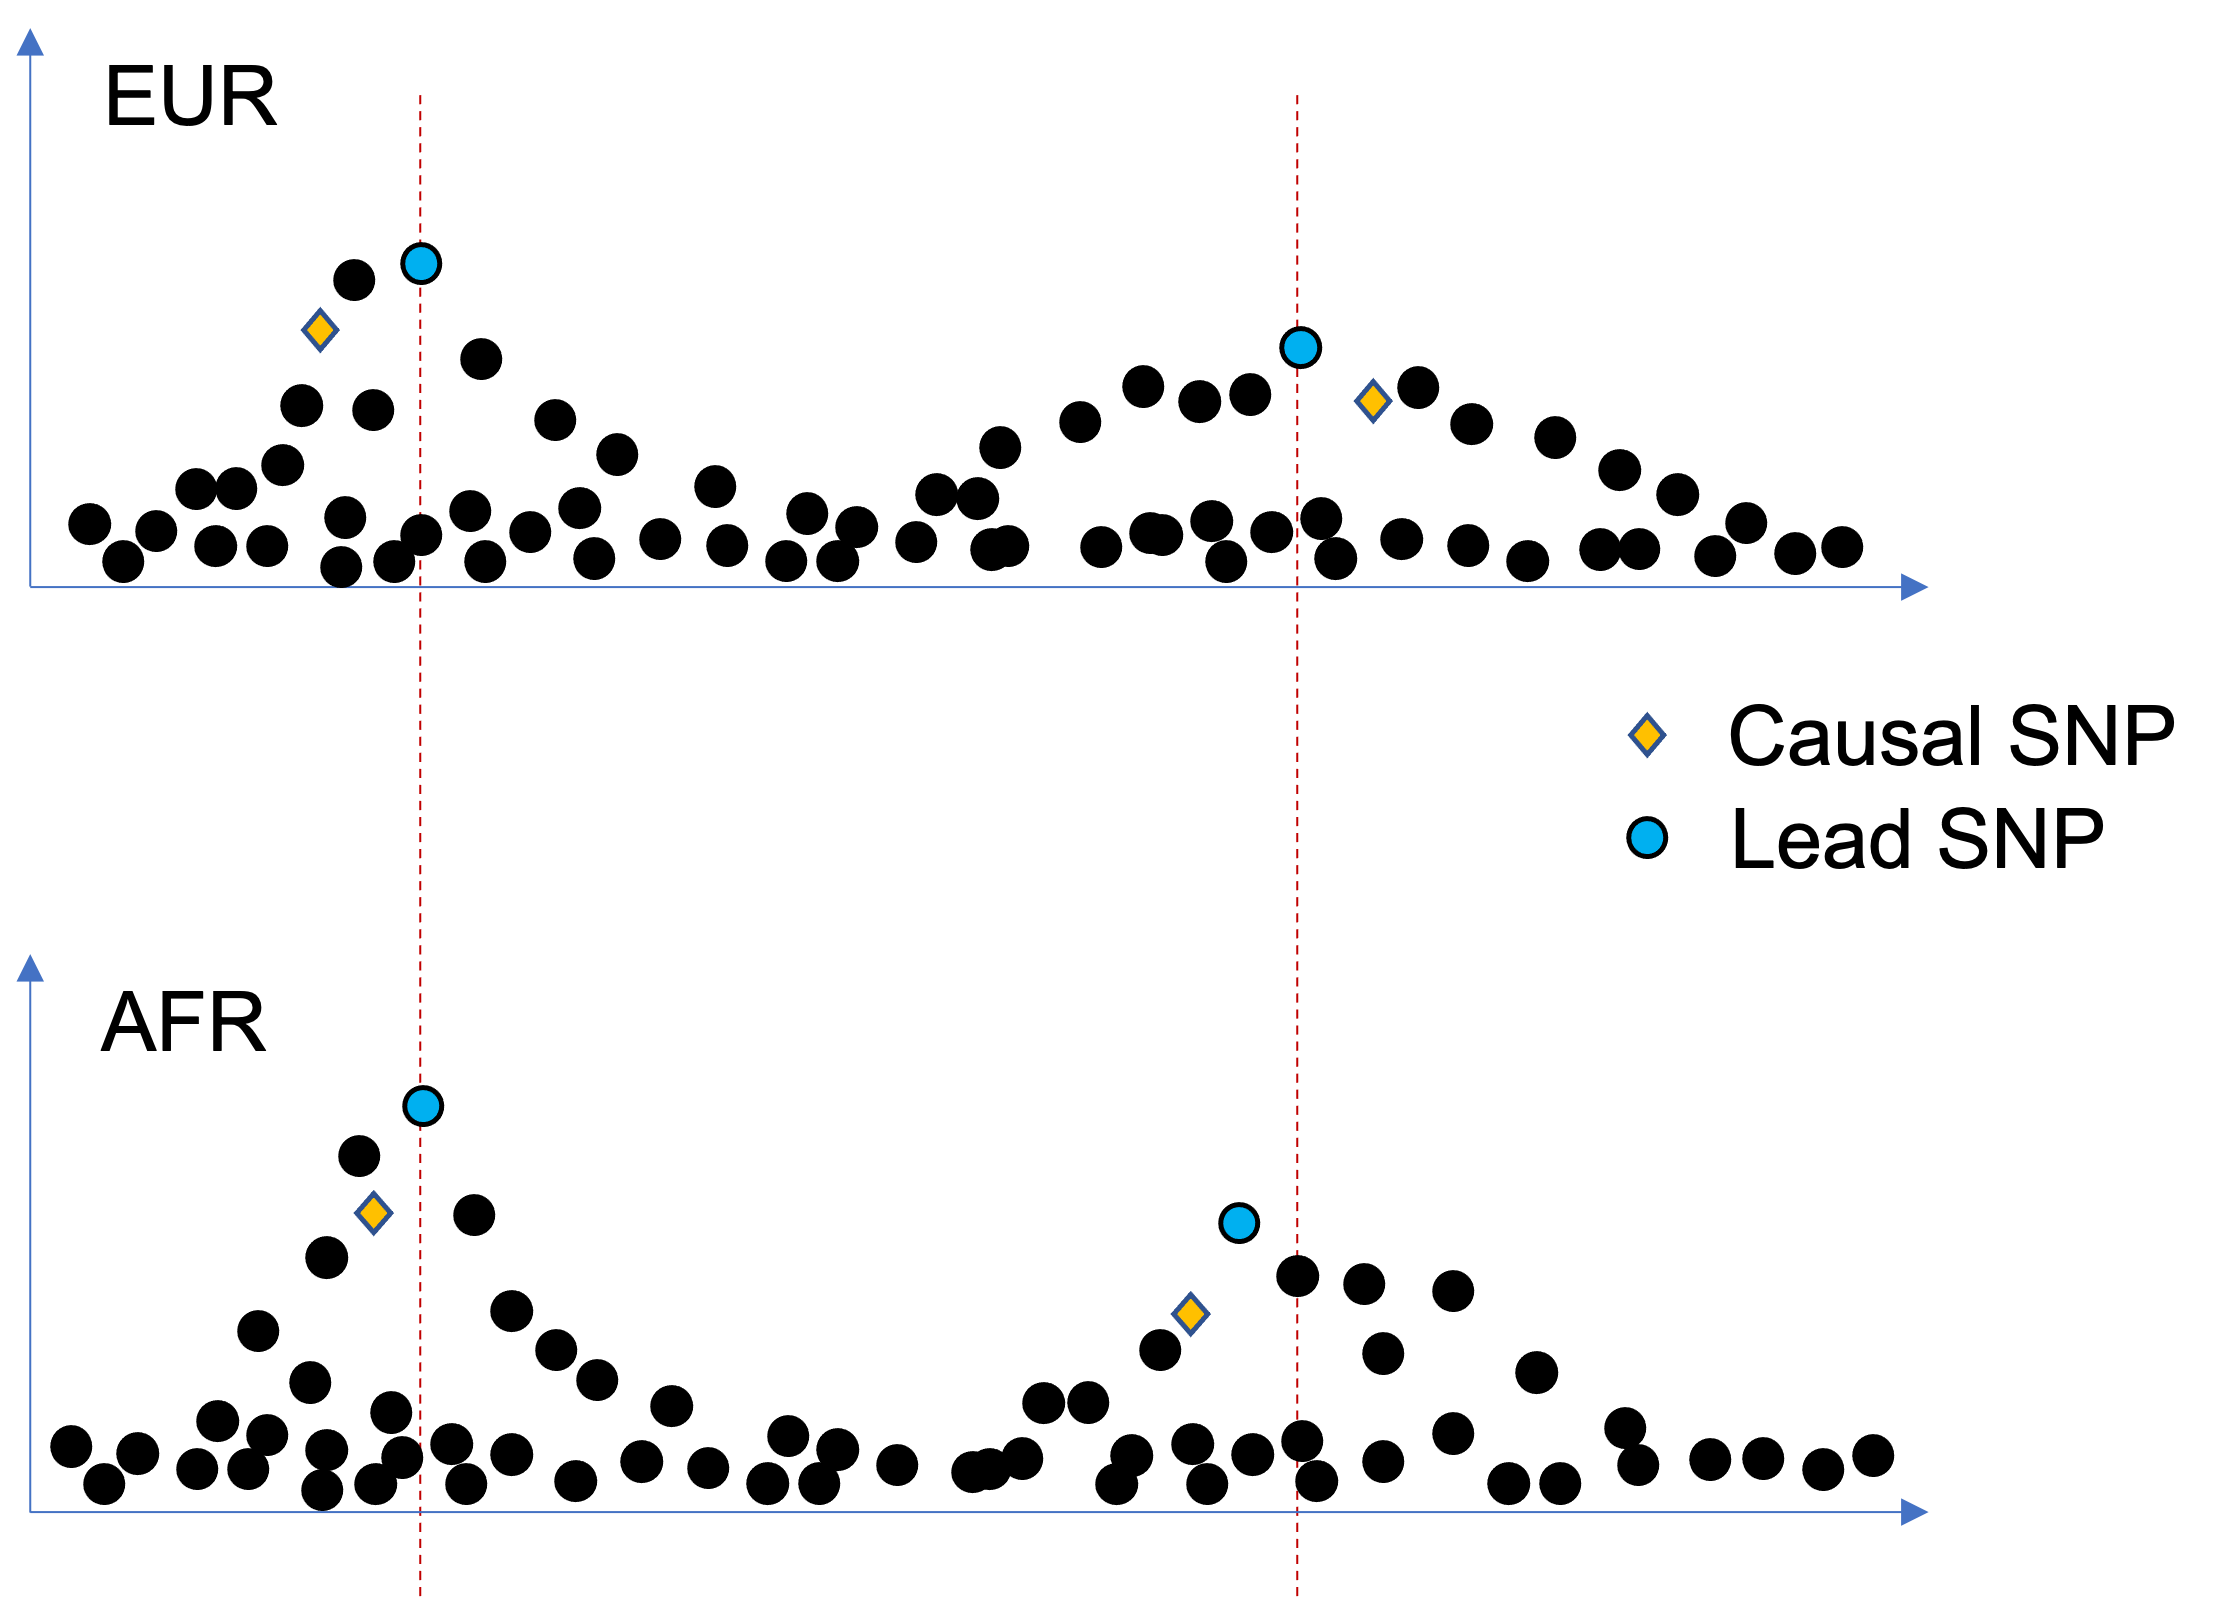
\includegraphics[width=.8\linewidth]{images/LD_similar.png}
  \caption{Similar LD blocks}
  \label{fig:Similar LD}
\end{subfigure}%
\begin{subfigure}{.5\textwidth}
  \centering
  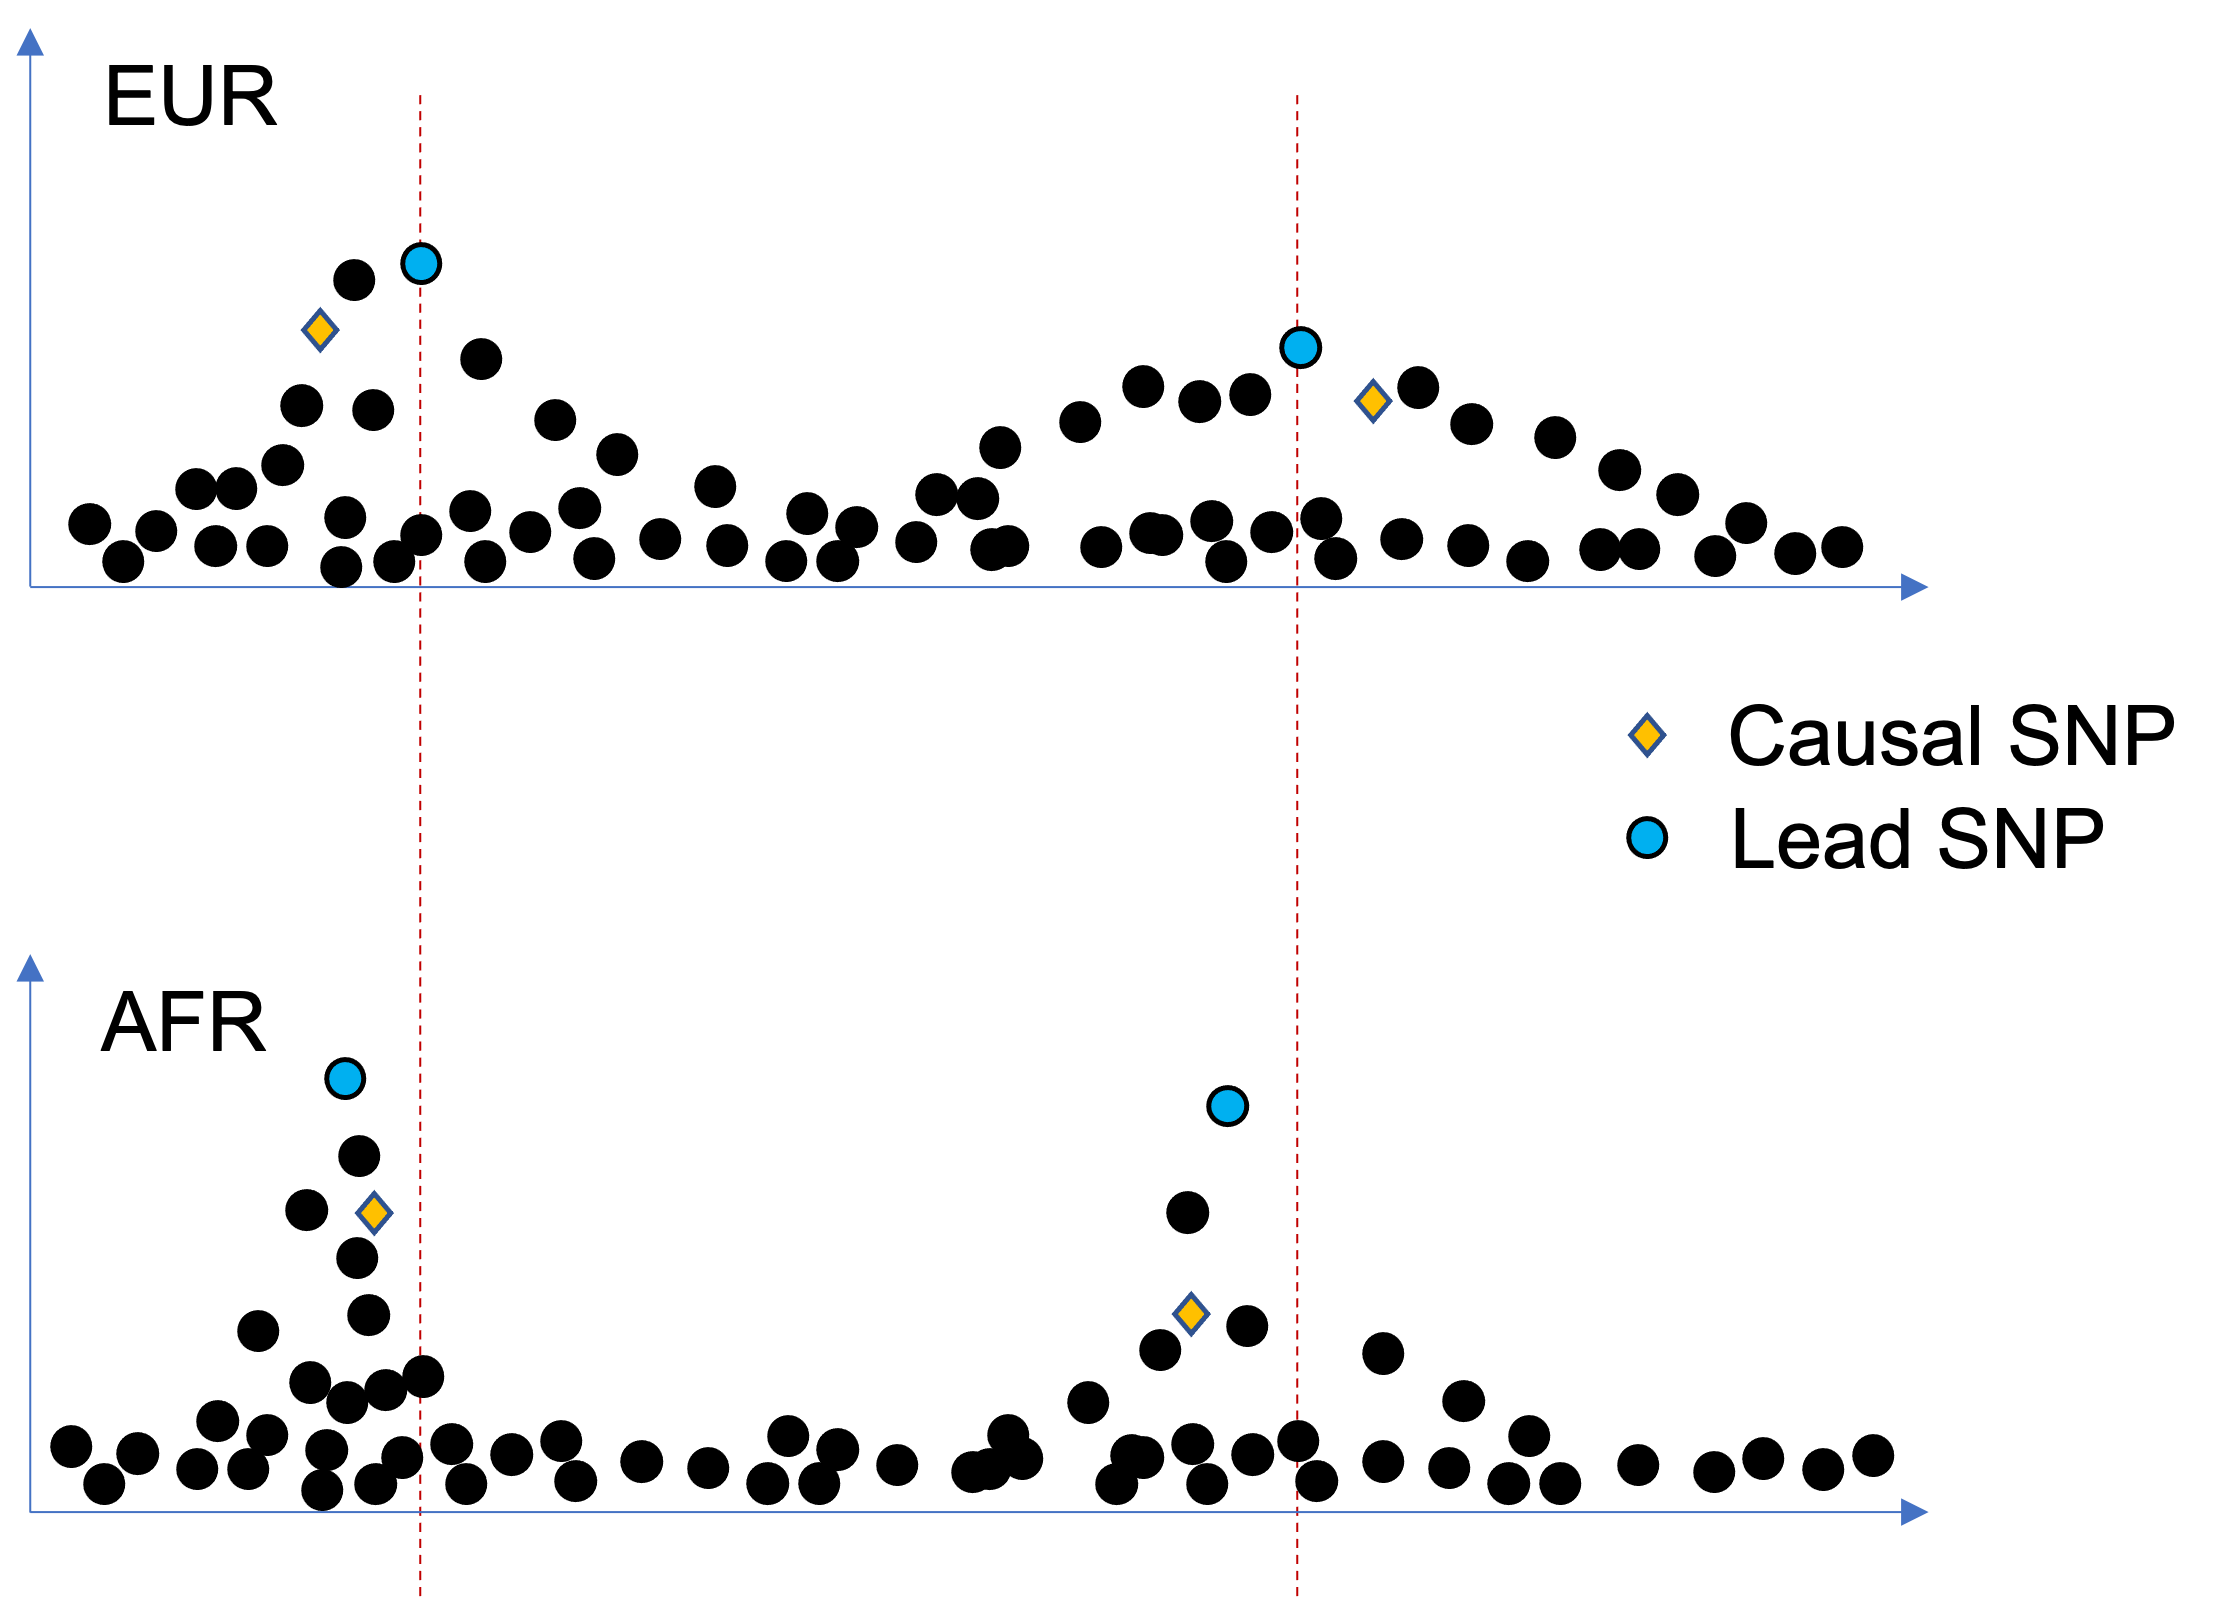
\includegraphics[width=.8\linewidth]{images/LD_diff.png}
  \caption{Different LD blocks}
  \label{fig:different LD}
\end{subfigure}
%\caption{A figure with two subfigures}
\label{fig:}
\end{figure}

\end{frame}

\begin{frame}{The Available Data}

\begin{itemize}
    \item The available training data is in summary statistics.  The correlation ($\boldsymbol{r}$) could be computed from the summary statistics.
    
    \begin{table}[h]
    \centering
    \tiny
    \begin{tabular}{|c c c c c c c c|} 
    \hline
       CHROME & POS & ID & REF & ALT & OR & SE & P\\ [0.5ex]
    \hline
    1 & 17407 & rs1570391677 & G & A & 1.034 & 0.034 & 0.337 \\
    1 & 54421 & rs1570391629 & A & G & 1.012 & 0.034 & 0.826 \\
    1 & 59615 & rs1639538192 & C & T & 1.051 & 0.034 & 0.365 \\
    1 & 108030 & rs1639538207 & G & T & 0.975 & 0.034 & 0.507 \\
    \hline
    \end{tabular}
    \end{table}
    \item The LD blocks ($\boldsymbol{R}$) can be obtained from available full genotype libraries, such as 1000 Genome Project.
\end{itemize}
    
\end{frame}

\begin{frame}{Lassosum: a penalized regression (LASSO) based method \citep{mak2017polygenic}}
%Lassosum: a penalized regression (LASSO) based method \citep{mak2017polygenic}.
lassosum is the building block of the proposed method.
It minimize the following objective function:
    $$
f(\boldsymbol{\beta})=\boldsymbol{y}^{T} \boldsymbol{y}+\boldsymbol{\beta}^{T} \boldsymbol{R} \boldsymbol{\beta}-2 \boldsymbol{\beta}^{T} \boldsymbol{r}+2 \lambda\|\boldsymbol{\beta}\|_{1}^{1}
     $$
\begin{itemize}
    \item $\lambda$ is the tuning parameter for LASSO penalty.
    \item $\boldsymbol{r}$ is a vector of correlations between SNPs and the phenotype, we only need summary statistics to get $\boldsymbol{r}$.
    \item $\boldsymbol{R}=\boldsymbol{X}^{T} \boldsymbol{X}$ is the correlations (LD) matrix.
    \item The data used to derive $\boldsymbol{R}$ and $\boldsymbol{r}$ are usually not the same.
\end{itemize}

%     \pause
%     As the genotype $\boldsymbol{X}$ used to derive LD is not the same in general as that for $\boldsymbol{r}$, use notation $\boldsymbol{R}=\boldsymbol{X}_r^{T}\boldsymbol{X}_r$
%     $$
%     f(\boldsymbol{\beta})=\boldsymbol{y}^{T} \boldsymbol{y}+\boldsymbol{\beta}^{T} \boldsymbol{X}_{r}^{T} \boldsymbol{X}_{r} \boldsymbol{\beta}-2 \boldsymbol{\beta}^{T} \boldsymbol{X}^{T} \boldsymbol{y}+2 \lambda\|\boldsymbol{\beta}\|_{1}^{]}
%     $$
%     This is no longer a penalized least square problem, replace $\boldsymbol{R}$ with $\boldsymbol{R}_{s}=(1-s) \boldsymbol{X}_{r}^{T} \boldsymbol{X}_{r}+s \boldsymbol{I}$, then it's equivalent to a LASSO problem
\end{frame}

\begin{frame}{The Proposed Method}

%Weighted regularized regression
$$
    \begin{aligned}
f(\boldsymbol{\beta})=&\gamma\left(\boldsymbol{y}^{T} \boldsymbol{y}+(1-s)\boldsymbol{\beta}^{T} \boldsymbol{R} \boldsymbol{\beta} - 2\boldsymbol{\beta}^{T} \boldsymbol{r} \right)\\
& + (1-\gamma)\left(\boldsymbol{y'}^{T} \boldsymbol{y'}+(1-s)\boldsymbol{\beta}^{T} \boldsymbol{R'} \boldsymbol{\beta} - 2 \boldsymbol{\beta}^{T} \boldsymbol{r'}\right)\\ 
& + s\boldsymbol{\beta}^{T}\boldsymbol{\beta} + 2
\sum_j\lambda|\beta_j|
    \end{aligned}
$$ 

\pause
\small 
\begin{itemize}
    \item $\gamma$ controls the balance between the two populations, $\lambda$ is the penalty tuning parameter and $s$ is a shrinkage parameter for ridge penalty.
    \pause
    \item The method calls for GWAS summary statistics ($\boldsymbol{r}$ and $\boldsymbol{r}^{'}$) and LD ($\boldsymbol{R}$ and $\boldsymbol{R}^{'}$) from two populations, with one population much bigger than the other. 
    \pause
    \item Leverage the genomics information from the bigger population, and inflate genomics information from the smaller population by $\gamma$
    \pause
    \item The objective function can be solved by coordinate descent algorithm. 
\end{itemize}
\end{frame}

%\begin{frame}{Figure illustration of the proposed method}
%  Insert a figure to intuitively illustrate our method.
    
%\end{frame}


\begin{frame}{Computation Efficiency}

\begin{figure}[h]	\noindent\makebox[\textwidth]{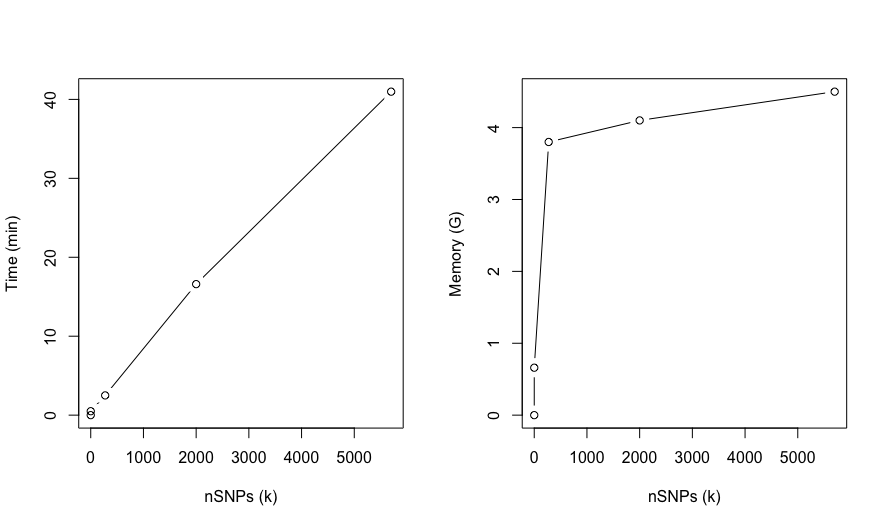
\includegraphics[scale=0.25]{images/benchmark.png}}
    %\caption{(A) Time vs nSNPs (B) Memory vs nSNPs}
    \label{fig:benchmark}
\end{figure}

\begin{itemize}
    \item I/O and matrix algebra functions are programmed by Rcpp. 
    \item Set a input data cap (default is 500Mb) to save memory. 
    \item The program can extract SNPs, their neighbours (within a specified distance in kb) and samples specified by user. 
\end{itemize}
    
\end{frame}



\begin{frame}{Tuning Parameters}
There are three tuning parameters (1) penalty parameter $\lambda$, (2) weighting parameter $\gamma$, and (3) shrinkage parameter $s$.

We would like to discuss model tuning in the following two scenarios
\begin{itemize}
    %\item Both genotype and phenotype for an independent testing data are available $\rightarrow$ simply compare AUC/R2 (ideal case)
    \item No independent tuning data is available (worst case).
    %\begin{itemize}
        %\item cross-validation: we can split the training data by cohorts/batches, if cohorts/batches specific summary statistics are available. 
        %\item  We hope that the AUC is not sensitive to gamma within a certain range (e.g. gamma vs AUC plot is flat when gamma is from 0.3 to 0.6). If this is true, we could argue that it is safe to pick a gamma from the range. Then given the picked gamma, select lambda by AIC/BIC. Extensive simulation are needed to give us reasonable ranges for different training data population ratios, signal levels and testing data population ratios.
    %\end{itemize}
    \item Summary statistics for an independent tuning data are available.
    \begin{itemize}
        \item Often the published results from a GWAS do not include individual  level information. Instead, summary statistics are published.
    \end{itemize}
\end{itemize}
\end{frame}

\begin{frame}{When Only Summary Statistics are Available}
We would like to minimize the distance between the predicted and true phenotype in testing data
$$
\ell=||\boldsymbol{y} - \boldsymbol{\tilede{\hat{y}}}||_2^2
$$
where $\boldsymbol{y}$ and $\boldsymbol{\hat{y}}$ are both normalized to unit norm. \\
\pause
\smallskip
After several steps of derivation, it can be approximated by 
$$
\ell= & 1 - \frac{\boldsymbol{\hat{\beta}}^{T} \boldsymbol{r}}{\sqrt{\hat{\boldsymbol{\beta}} (\boldsymbol{R}/n) \hat{\boldsymbol{\beta}}}}
$$
where $\boldsymbol{r}$ can be calculated from GWAS summary statistics, and $\boldsymbol{R}$ is the LD matrix.
\end{frame}

\begin{frame}{Simulation Study I}
%Insert diagrams to show the simulation settings below
\begin{itemize}
    \item GWAS summary statistics: 20,000 Europeans (EUR), plus 2,000, 4,000 , 8,000 or 20,000 Africans (AFR)
    \item LD information: 2,000 EUR, 2,000 AFR 
    \item Tuning data: 4,000 AFR
    \item Testing data: 4,000 AFR
    \item 5.7 million SNPs, 300 causal SNPs
    %\item Signal (beta): x1, x3, x5, x10
\end{itemize}
\end{frame}

\begin{frame}{Parameter Tuning}
\begin{figure}[h]	\noindent\makebox[\textwidth]{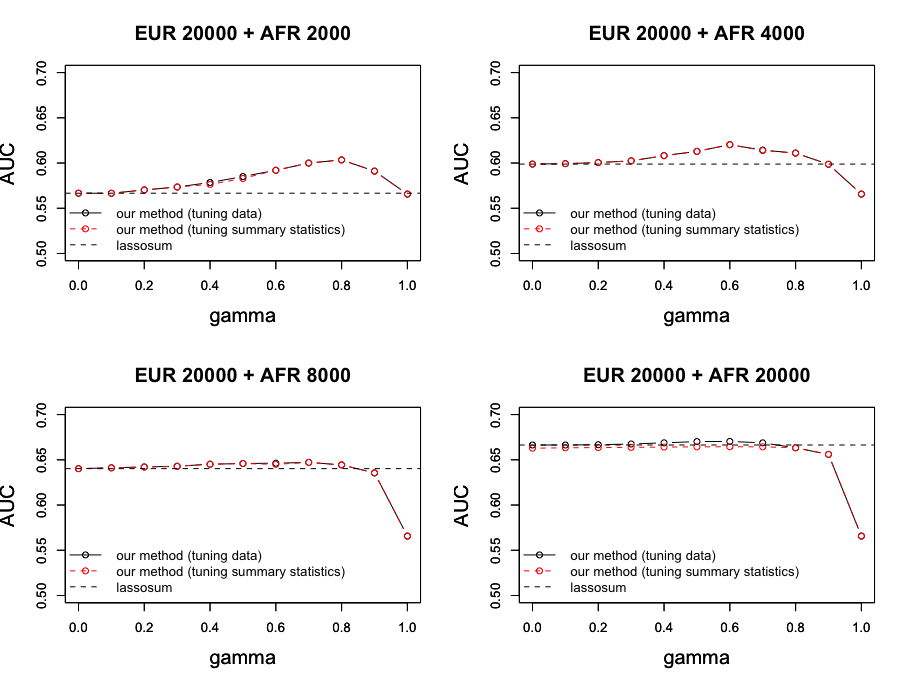
\includegraphics[scale=0.32]{images/Modeltuning.png}}
      %\caption{gamma vs AUC}
      \label{fig:modeltuning_gamma_vs_AUC}
\end{figure}
\end{frame}


\begin{frame}{Simulation Study II}
%Insert diagrams to show the simulation settings below
\begin{itemize}
    \item Whole genome: ~5.7 million SNPs, 4000 causal SNPs
    \item Simulated datasets for Europeans (EUR) and Africans (AFR)
    \begin{itemize}
    \item GWAS summary statistics: 20,000 EUR, 4,000 AFR
    \item A separate data for LD information
    \item Tuning data
    \item Testing data
    \end{itemize}

    %\item Signal (beta): x1, x3, x5, x10
\end{itemize}
\end{frame}

\begin{frame}{Prediction: The Proposed Method vs Lassosum}

\begin{figure}[h]	\noindent\makebox[\textwidth]{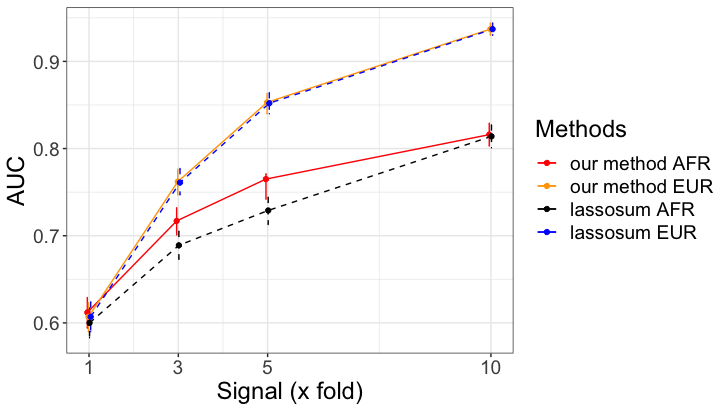
\includegraphics[scale=0.35]{images/AUC_our_vs_lassosum.png}}
      \label{fig:our-EUR vs our-AFR}
\end{figure}
\begin{itemize}
    \item The proposed method improves performance for both AFR and EUR testing data.
    \item The improvement depends on the level of causal SNP effects.
\end{itemize}
\end{frame}

\begin{frame}{Prediction: Comparing Multiple Methods}
%Insert diagrams to show the simulation settings below
\begin{figure}[h]	
\noindent\makebox[\textwidth]{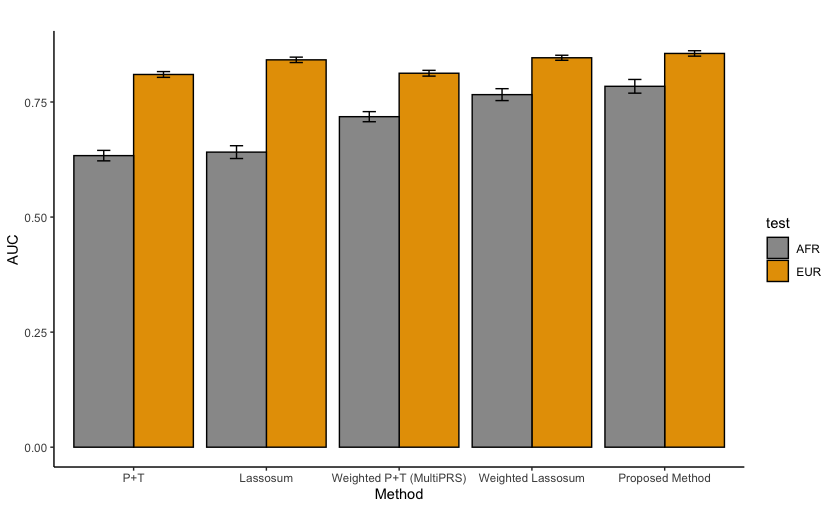
\includegraphics[scale=0.3]{images/methods_comparison.png}}
      %\caption{gamma vs AUC}
   \label{fig:methods comparison}
\end{figure}

\begin{itemize}
    %\item Leveraging information from the smaller population can improve performance of the original method.
    %\item The proposed method performs best for testing data of both populations
    \item MultiPRS (weighted P+T): $PRS_{combined} = \alpha PRS_{EUR} + (1-\alpha) PRS_{AFR}$
    \item Weighted lassosum: same idea can be extended to lassosum
\end{itemize}

\end{frame}


\begin{frame}{Disparities in Lassosum}

\begin{figure}[h]	
\noindent\makebox[\textwidth]{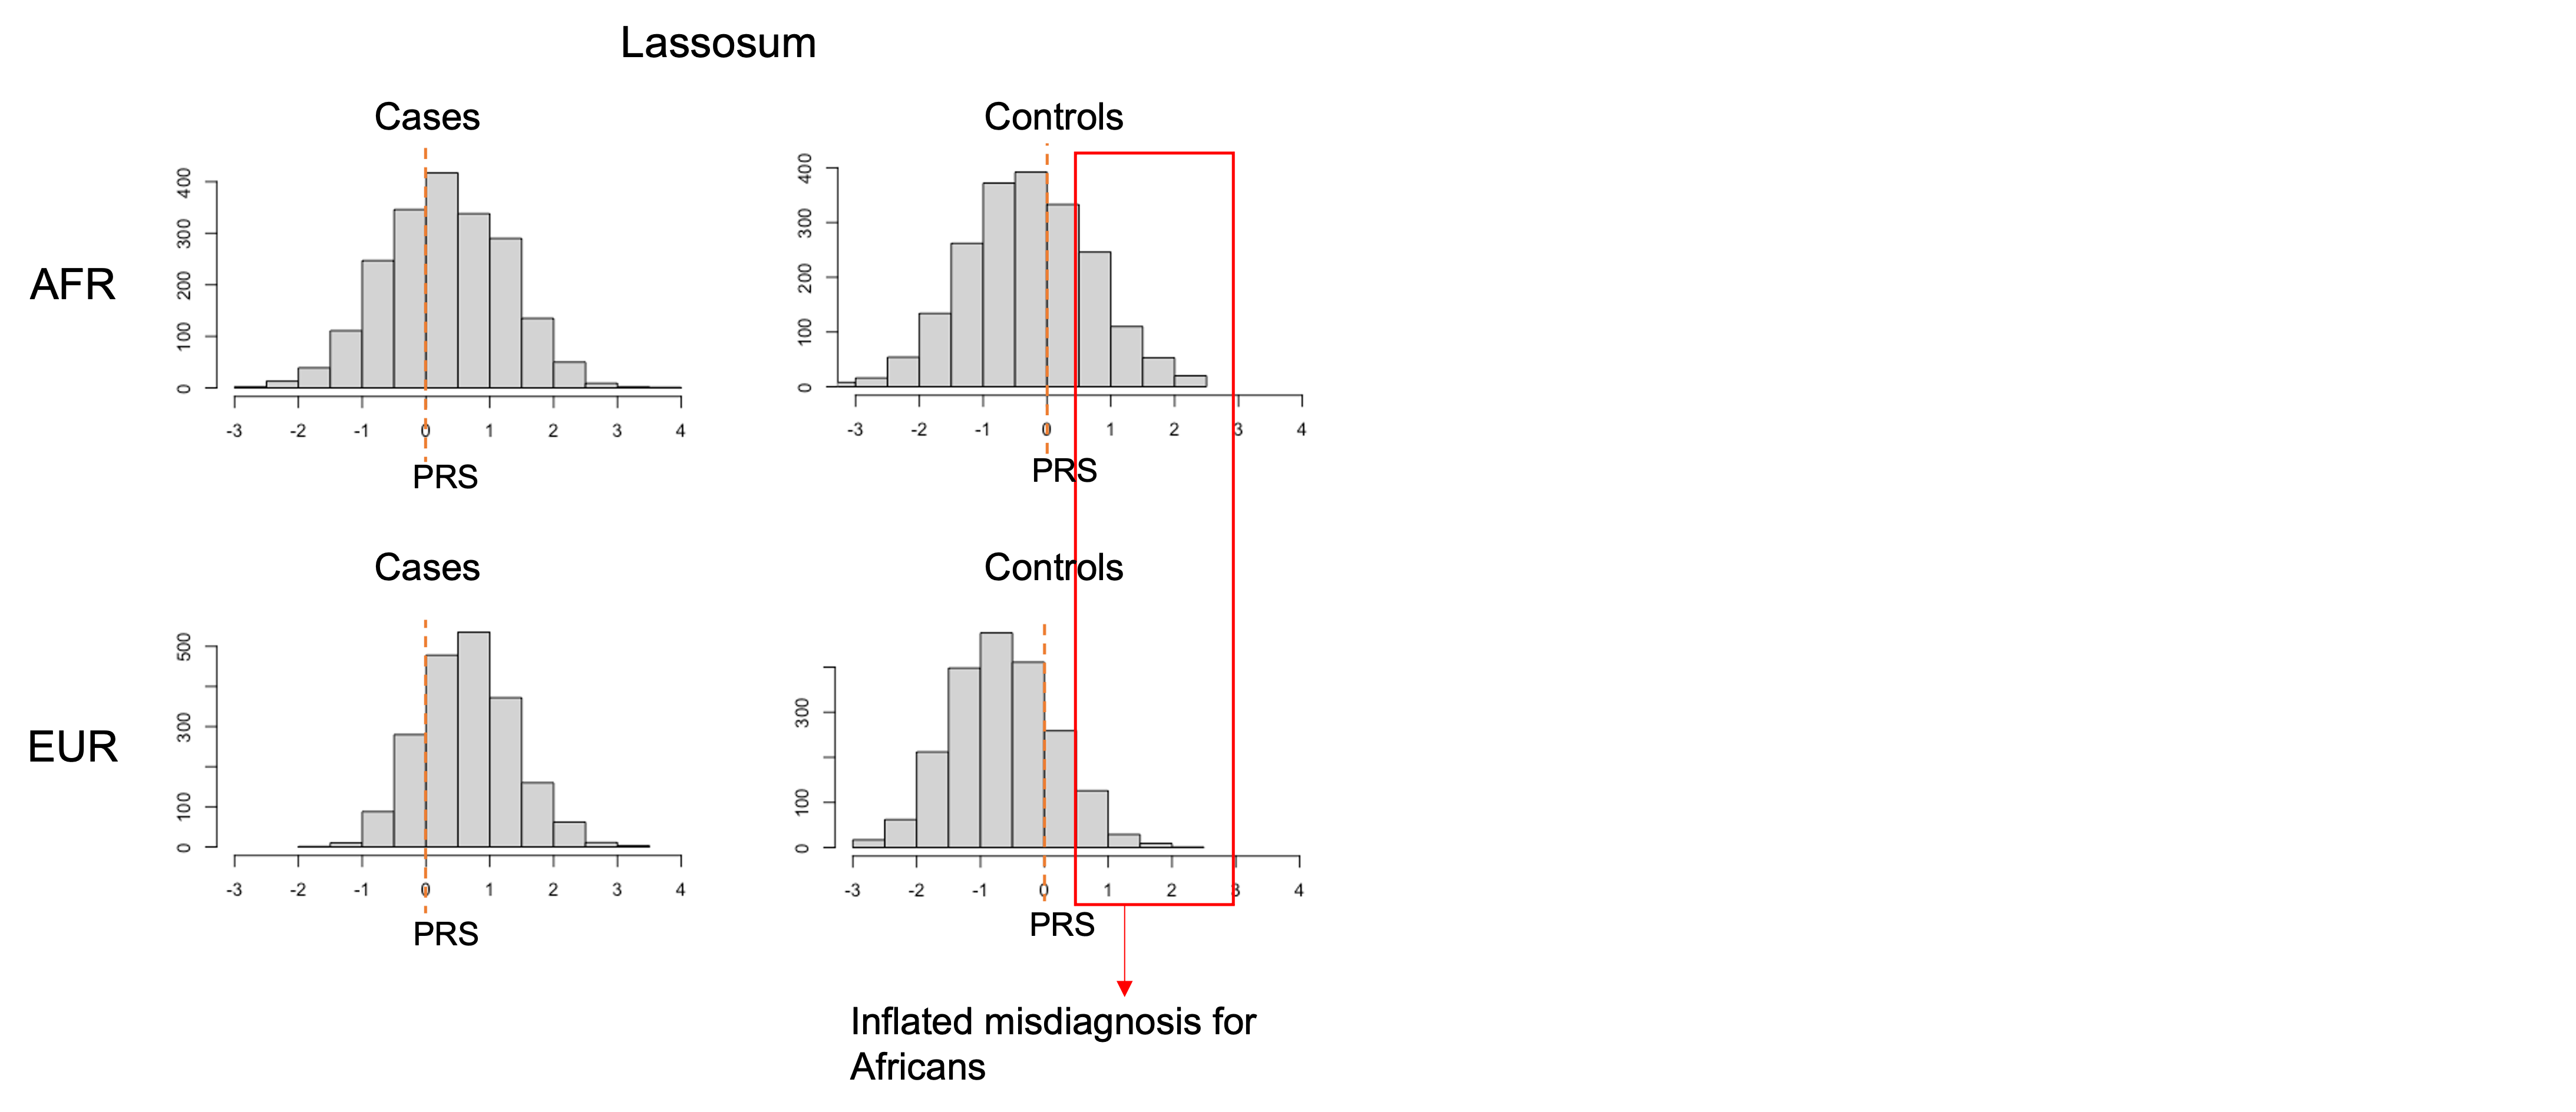
\includegraphics[scale=0.35]{images/lassosum_disparities1.png}}
      %\caption{gamma vs AUC}
   \label{fig:lassosum disparities}
\end{figure}

%Our method mitigate the disparities in the number of false positives by lassosum in simulation study.
\end{frame}

\begin{frame}{Disparities in Lassosum}

\begin{figure}[h]	
\noindent\makebox[\textwidth]{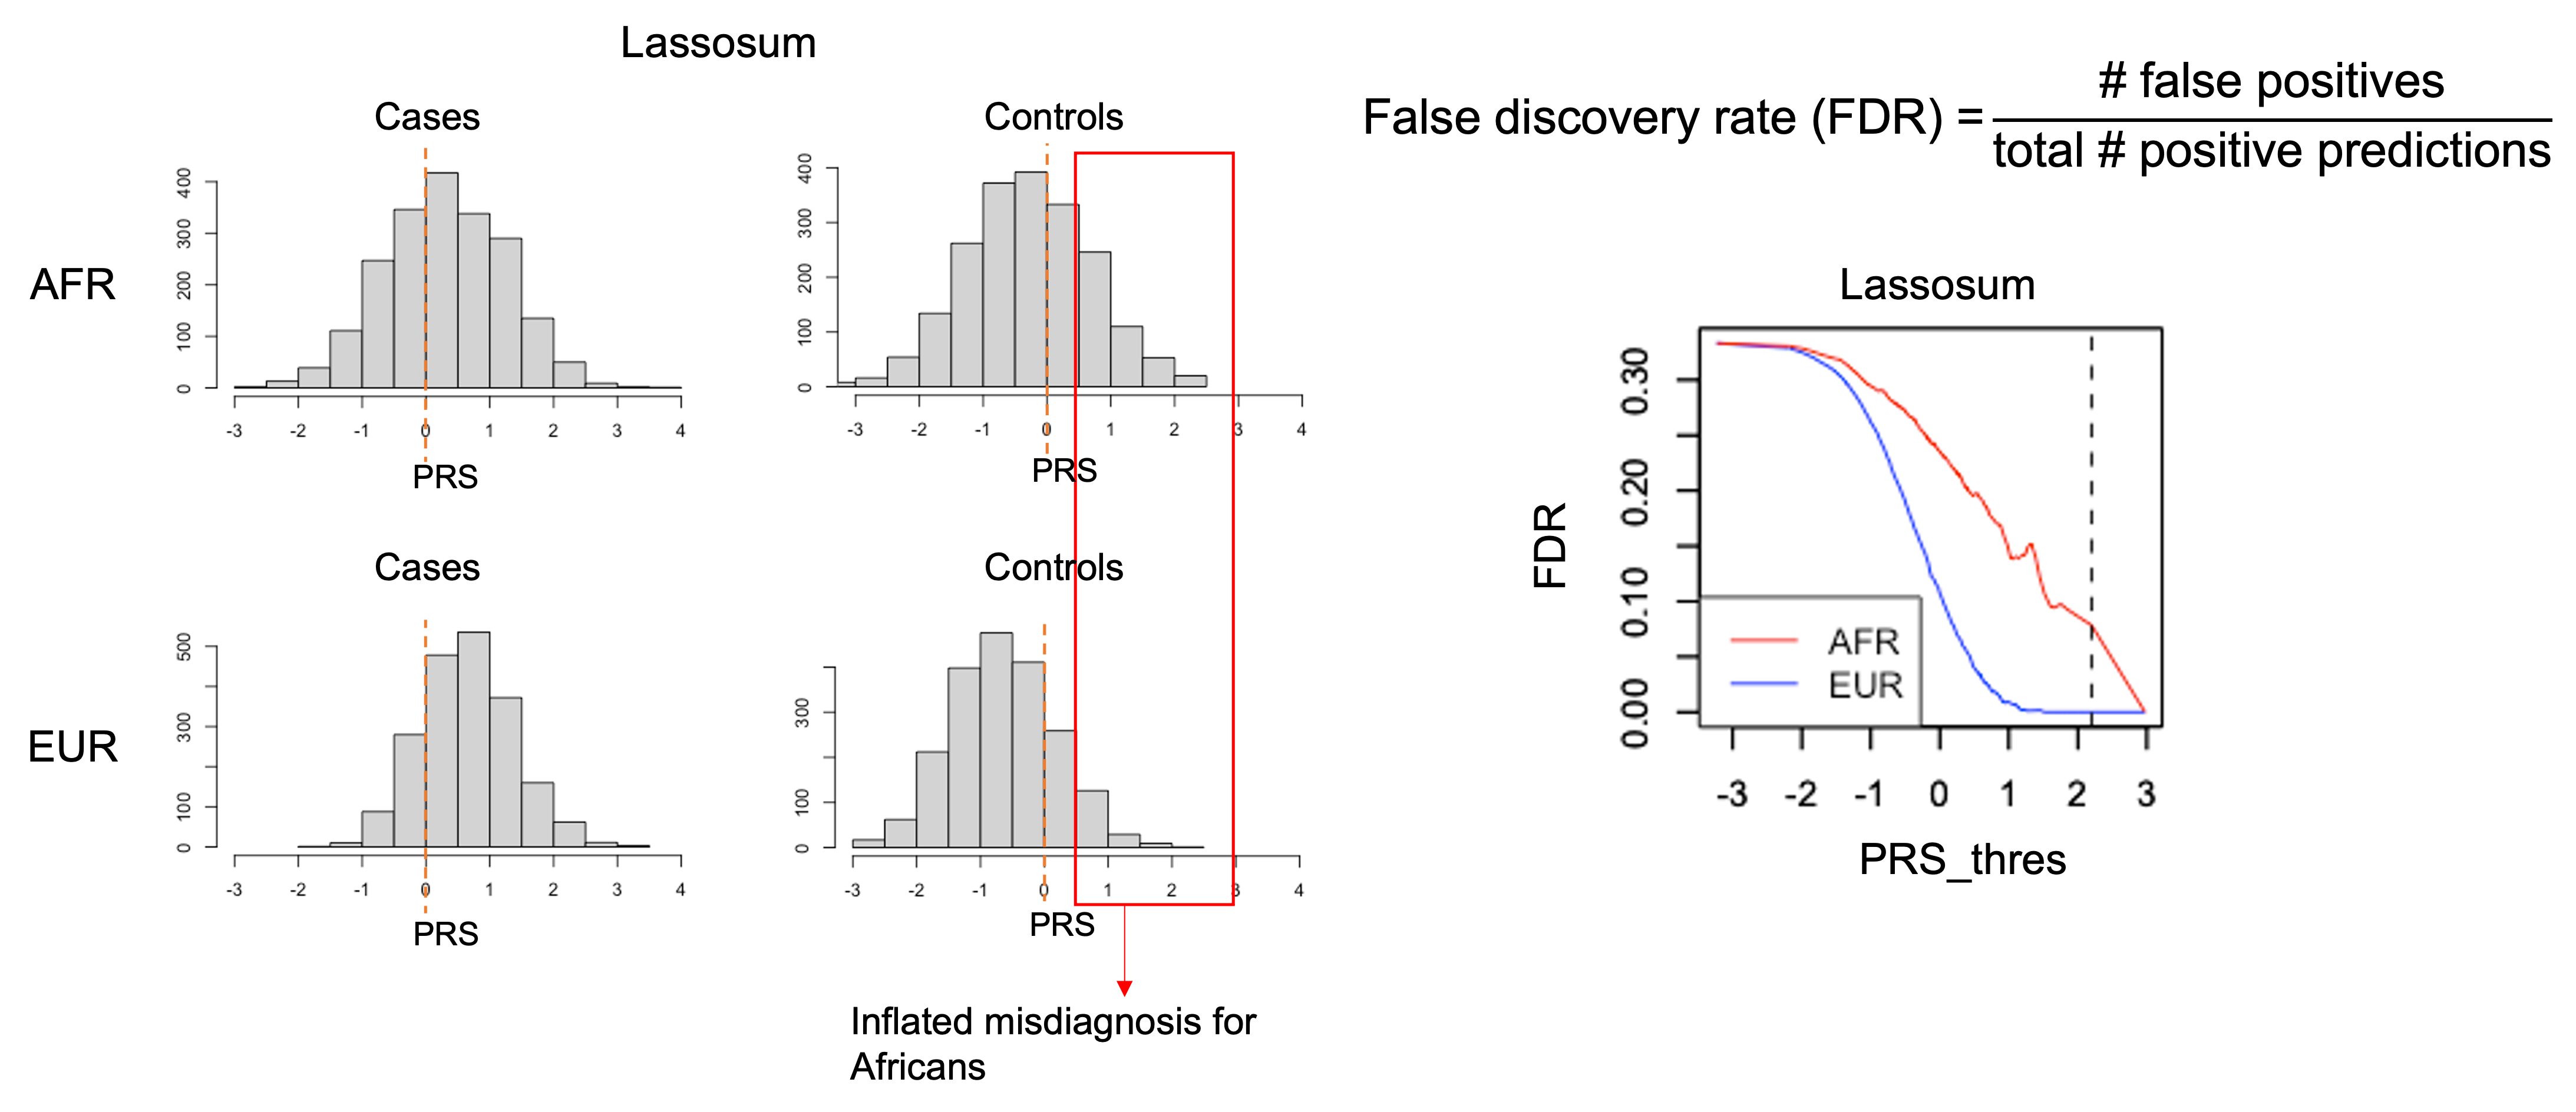
\includegraphics[scale=0.35]{images/lassosum_disparities2.png}}
      %\caption{gamma vs AUC}
   \label{fig:lassosum disparities}
\end{figure}

%Our method mitigate the disparities in the number of false positives by lassosum in simulation study.
\end{frame}

\begin{frame}{Racial Disparities in Schizophrenia Diagnosis}

\begin{itemize}
    \item African-Americans are more likely to be misdiagnosed as having schizophrenia, which has been reported by numerous studies.
        \begin{itemize}
            \item    In a 2018 analysis of data from 52 different studies, \cite{olbert2018meta} found that African-Americans are 2.4 times more likely to be diagnosed with schizophrenia. \\
            \item \cite{schwartz2014racial} claim it's 3-4 times higher
            \item Improved PRS might help with diagnosis bias.
        \end{itemize}
\end{itemize}

\end{frame}

\begin{frame}{The Proposed Method Mitigates the Disparities}

\begin{figure}[h]	\noindent\makebox[\textwidth]{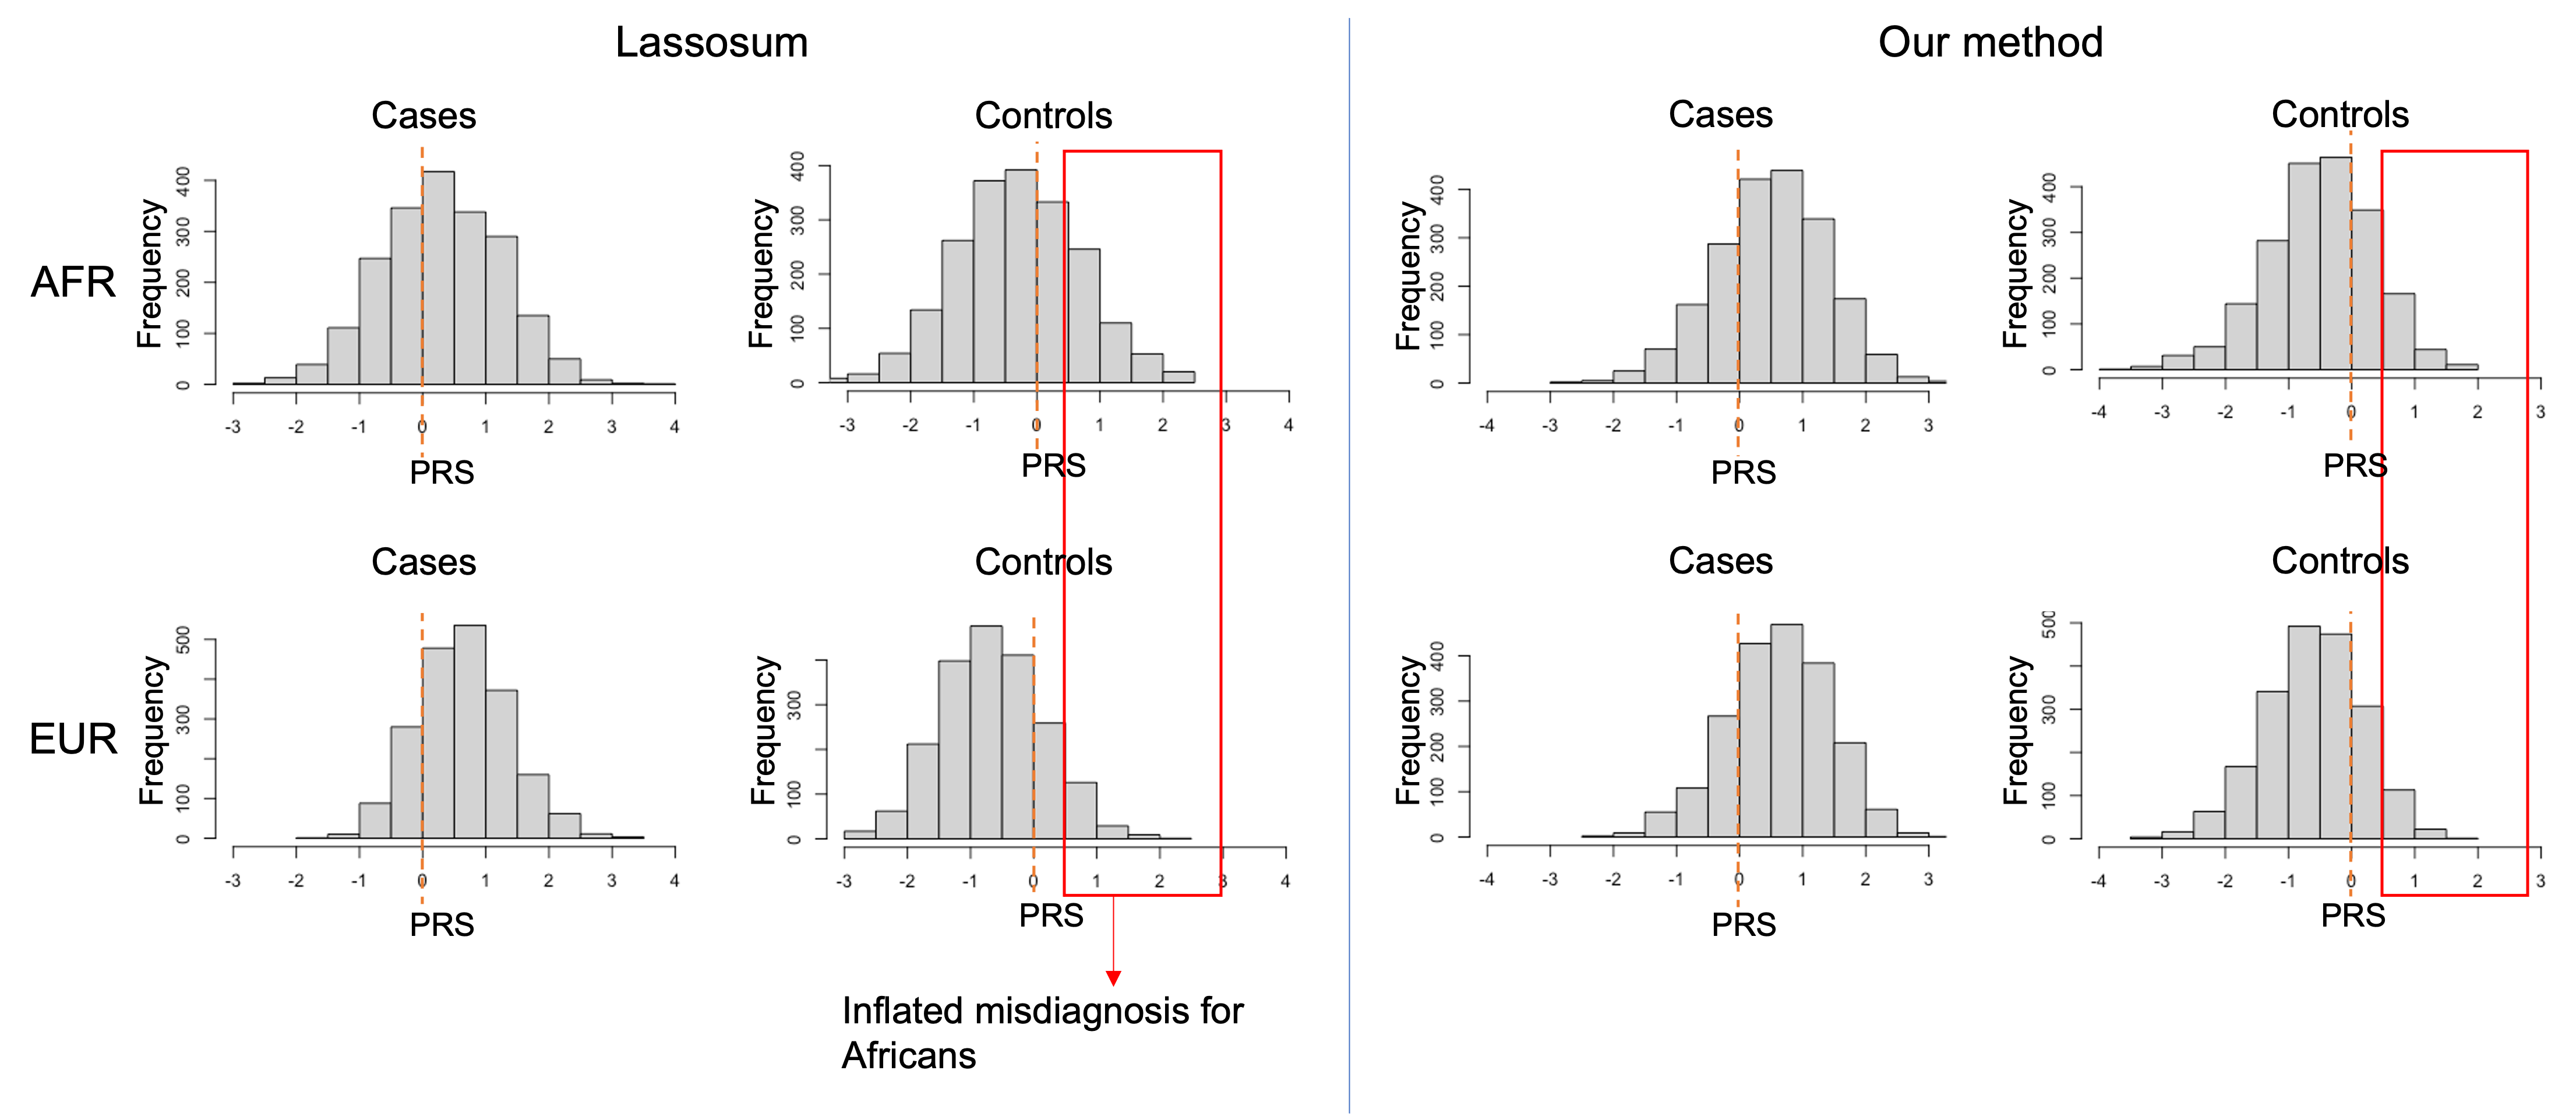
\includegraphics[scale=0.35]{images/Histogram.png}}
              \label{fig:Histogram}
\end{figure}

The proposed method mitigates the disparities in the number of false positives by lassosum in simulation studies.
\end{frame}

\begin{frame}{The Proposed Method Mitigates the Disparities}
%\begin{itemize}
    %\item False Positive rate (FPR): $\text{FPR} =\frac{\text{\# false positives}}{\text{\# controls}}$ 
%\begin{figure}[h]	\noindent\makebox[\textwidth]{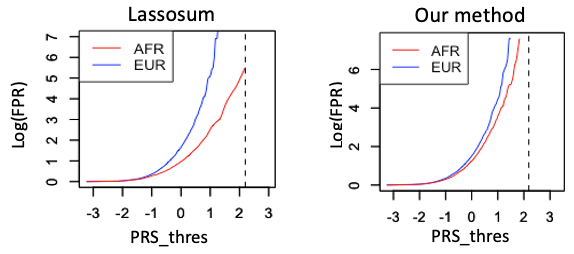
\includegraphics[scale=0.3]{images/FPR.png}}
%              \label{fig:FPR and FDR}
%\end{figure}

False discovery rate (FDR): $\text{FDR} =\frac{\text{\# false positives}}{\text{\# positive predictions}}$ 
%= \# false positives / total \# positive predictions
\begin{figure}[h]	\noindent\makebox[\textwidth]{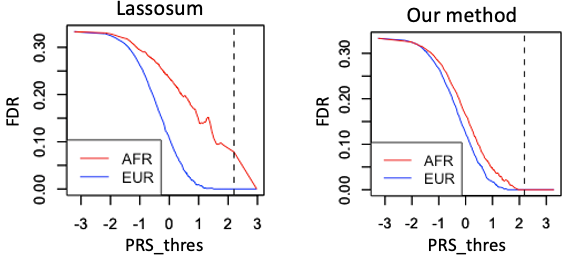
\includegraphics[scale=0.4]{images/FDR.png}}
              \label{fig:FPR and FDR}
\end{figure}
%\end{itemize}
\end{frame}



%\begin{frame}{Methods Comparison in Simulation Studies}

%\begin{figure}[h]	
%\noindent\makebox[\textwidth]{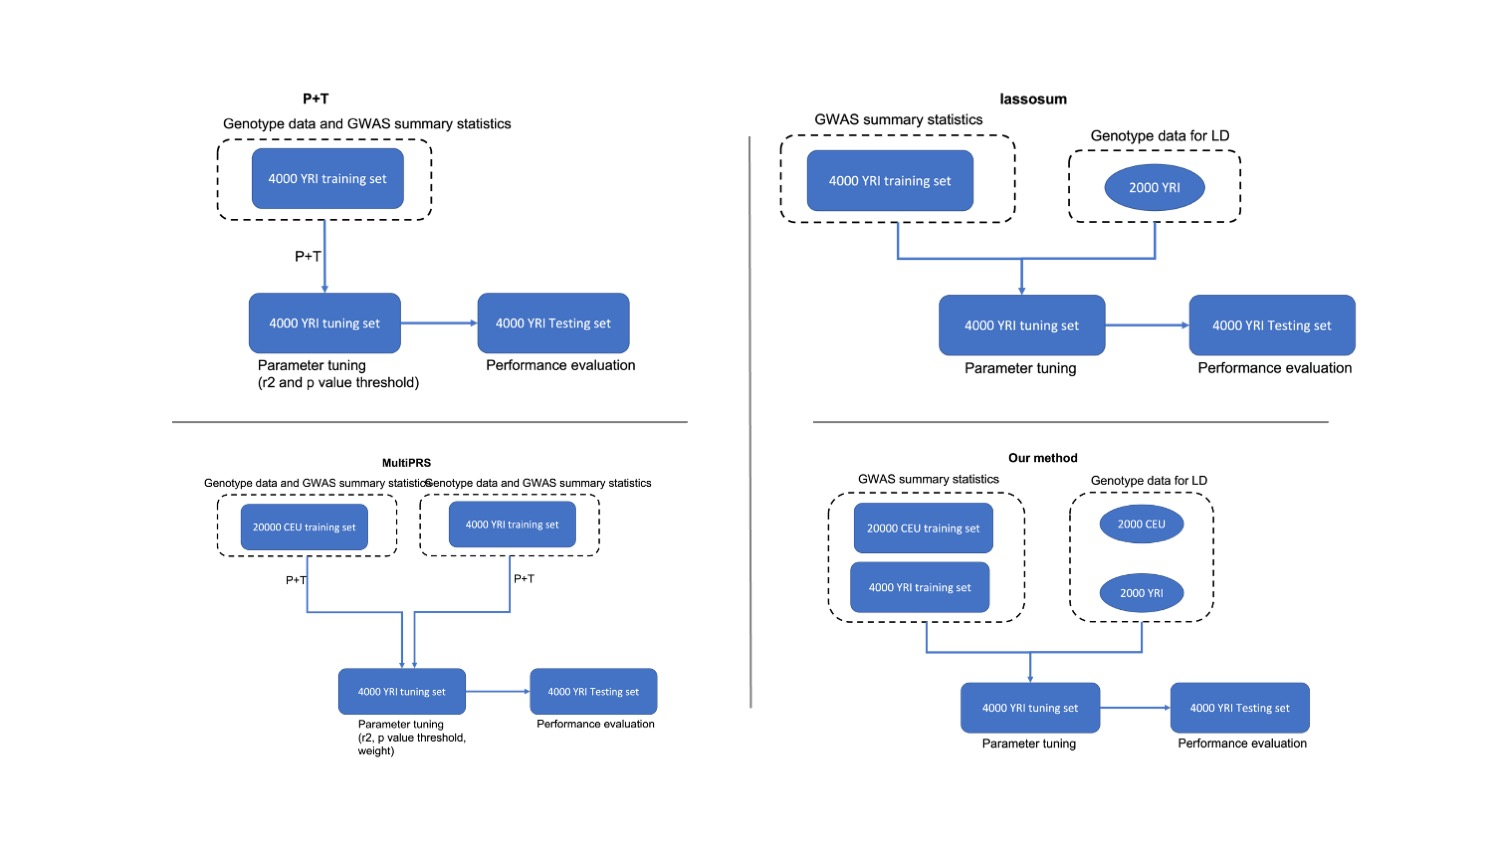
\includegraphics[scale=0.25]{images/Setting.jpg}}
      %\caption{gamma vs AUC}
%   \label{fig:methods comparison}
%\end{figure}

%\end{frame}

%\begin{frame}{Methods Comparison in Simulation Studies}
%Will insert Bert's result once we have it
%\begin{figure}[h]	
%\noindent\makebox[\textwidth]{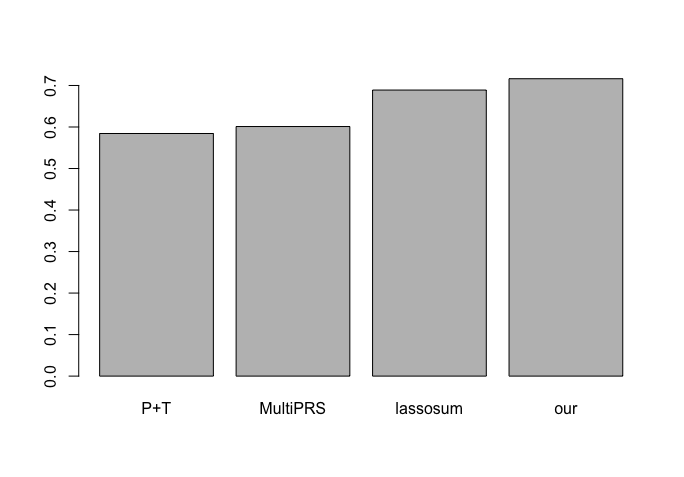
\includegraphics[scale=0.4]{images/comparison.AUC.png}}
      %\caption{gamma vs AUC}
%   \label{fig:methods comparison}
%\end{figure}

%\end{frame}

%\begin{frame}{Methods Comparison in Simulation Studies}
%Will insert a figure comparing disparities.

%\end{frame}

%\begin{frame}{Real data application}
    
%\end{frame}

\begin{frame}{Summary}
    \begin{itemize}
        \item We have developed a novel statistical method for PRS by incorporating genetic information from two ancestries.
        \item The proposed method jointly estimates the effect size and choose the SNPs that are predictive for both ancestries.
        \item The proposed method improves trans-ancestry portability of PRS.
        \item The proposed method could mitigate the disparities in the diagnosis of schizophrenia.
    \end{itemize}
\end{frame}

\begin{frame}{Future Direction}
\begin{itemize}
    \item Apply our method to admixed population.
    \item Can we borrow information from Autism to predict the patients with schizophrenia? 
    \item How to integrate genetic and clinical risk?
\end{itemize}
\end{frame}

\begin{frame}{Acknowledgement}
    \begin{itemize}
        \item Kathryn
        \item Bernie
        \item Max
        \item Bert
    \end{itemize}
\end{frame}

\begin{frame}
    \bibliography{ref.bib}
    \bibliographystyle{apalike}
\end{frame}

    
\begin{frame}{Lassosum: a penalized regression (LASSO) based method \citep{mak2017polygenic}}
    Proof: \\
    $\boldsymbol{R}_{s}=(1-s) \boldsymbol{X}_{r}^{T} \boldsymbol{X}_{r}+s \boldsymbol{I}$ is positive definite, and there is always exit $\boldsymbol{W}$ and $\boldsymbol{v}$ such that $\boldsymbol{W}^{T} \boldsymbol{W}=\boldsymbol{R}_{s}, \quad \boldsymbol{W}^{T} \boldsymbol{v}=\boldsymbol{r}$.\\
    
    %\pause
    
    So the objective function becomes:
    $$
    \begin{aligned}
    f(\boldsymbol{\beta})=& \boldsymbol{y}^{T} \boldsymbol{y}+(1-s) \boldsymbol{\beta}^{T} \boldsymbol{X}_{r}^{T} \boldsymbol{X}_{r} \boldsymbol{\beta}-2 \boldsymbol{\beta}^{T} \boldsymbol{r} \\
    &+s \boldsymbol{\beta}^{T} \boldsymbol{\beta}+2 \lambda\|\boldsymbol{\beta}\|_{1}^{1},
    \end{aligned}
    $$   
    when $0 < s < 1$, the objective function could be solved using the method for elastic net problem by coordinate descent algorithms, avoiding computationally expensive LD matrix $\boldsymbol{X}_r^T\boldsymbol{X}_r$ calculation.
\end{frame}

\begin{frame}{Coordinate Descent Algorithm}
\begin{itemize}
    \item It’s reasonable to assume the SNPs from different LD blocks are not correlated. For computational efficiency, we would like to compute the gradient at $\beta_j$ by its corresponding LD blocks. \\
    \item The coodinate-wise update for $\beta_j$ is
\begin{equation}
    \beta_{j}= \begin{cases}0 & \text { otherwise } \\ \frac{\text{ sign}(u_j)(\left|u_j\right| - \lambda)}{\gamma \tilde{\boldsymbol{X}}_{j}^{T} \tilde{\boldsymbol{X}}_{j} + (1-\gamma) \tilde{\boldsymbol{X'}}_{j}^{T} \tilde{\boldsymbol{X'}}_{j} + s} & \text { if }\left|u_j\right| > \lambda \end{cases}
    \label{equation_update_beta}
\end{equation}
where $u_j=\gamma \left(r_{j}-\tilde{\boldsymbol{X}}_{j}^{T} \tilde{\boldsymbol{X}}_{-j}^{[k]} \tilde{\boldsymbol{\beta}}_{-j}^{[k]}\right) + (1-\gamma) \left(r'_{j}-\tilde{\boldsymbol{X'}}_{j}^{T} \tilde{\boldsymbol{X'}}_{-j}^{[k']} \tilde{\boldsymbol{\beta}}_{-j}^{[k']}\right)$
\end{itemize}
\end{frame}

\begin{frame}{Coordinate Descent Algorithm}
\begin{itemize}
    \item It’s reasonable to assume the SNPs from different LD blocks are not correlated. For computational efficiency, we would like to compute the gradient at $\beta_j$ by its corresponding LD blocks. \\
    \item The coodinate-wise update for $\beta_j$ is
\begin{equation}
    \beta_{j}= \begin{cases}0 & \text { otherwise } \\ \frac{\text{ sign}(u_j)(\left|u_j\right| - \lambda)}{\gamma \tilde{\boldsymbol{X}}_{j}^{T} \tilde{\boldsymbol{X}}_{j} + (1-\gamma) \tilde{\boldsymbol{X'}}_{j}^{T} \tilde{\boldsymbol{X'}}_{j} + \tikzmark{c1}s\tikzmark{c2}} & \text { if }\left|u_j\right| > \lambda \end{cases}
    \label{equation_update_beta}
\end{equation}
where $u_j=
\gamma \tikzmark{a1} \left(r_{j}-\tilde{\boldsymbol{X}}_{j}^{T} \tilde{\boldsymbol{X}}_{-j}^{[k]} \tilde{\boldsymbol{\beta}}_{-j}^{[k]}\right) 
\tikzmark{a2}
+ 
 (1-\gamma) \tikzmark{b1} \left(r'_{j}-\tilde{\boldsymbol{X'}}_{j}^{T} \tilde{\boldsymbol{X'}}_{-j}^{[k']} \tilde{\boldsymbol{\beta}}_{-j}^{[k']}\right)
\tikzmark{b2}
$
    \begin{tikzpicture}[overlay,remember picture,
box/.style = {rounded corners, fill=#1},
pin edge={-Stealth,thick, red}
                        ]
\coordinate (A1) at ($({pic cs:a1})+(+0.5ex, 3ex)$);
\coordinate (A2) at ($({pic cs:a2})+(-0.5ex,-2ex)$);
\coordinate (B1) at ($({pic cs:b1})+(+0.5ex, 3ex)$);
\coordinate (B2) at ($({pic cs:b2})+(-0.5ex,-2ex)$);
\coordinate (C1) at ($({pic cs:c1})+(+0.5ex, 0.5ex)$);
\coordinate (C2) at ($({pic cs:c2})+(-0.5ex,-0.5ex)$);
\node[box=blue!30,semitransparent,
      fit=(A1) (A2),
      pin=below:\alert{Ancestry 1}]  {};
\node[box=red!30,semitransparent,
      fit=(B1) (B2),
      pin=below:\alert{Ancestry 2}]  {};
\node[box=green!10,semitransparent,
      fit=(C1) (C2),
      pin=right:\alert{\small{shrinkage parameter}}]  {};     
\end{tikzpicture}

\end{itemize}
\end{frame}

\begin{frame}{Simulation Study III}
%Insert diagrams to show the simulation settings below
\begin{itemize}
\tiny
    \item GWAS summary statistics: 20,000 Europeans (EUR), 4,000 Africans (AFR)
    \item LD information: 5,000 EUR, 5,000 AFR 
    %\item Tuning data: 4,000 AFR
    \item Testing data: ? AFR and ? EUR
    \item ~5.7 million SNPs, 4000 causal SNPs
\end{itemize}

\begin{figure}[h]	
\noindent\makebox[\textwidth]{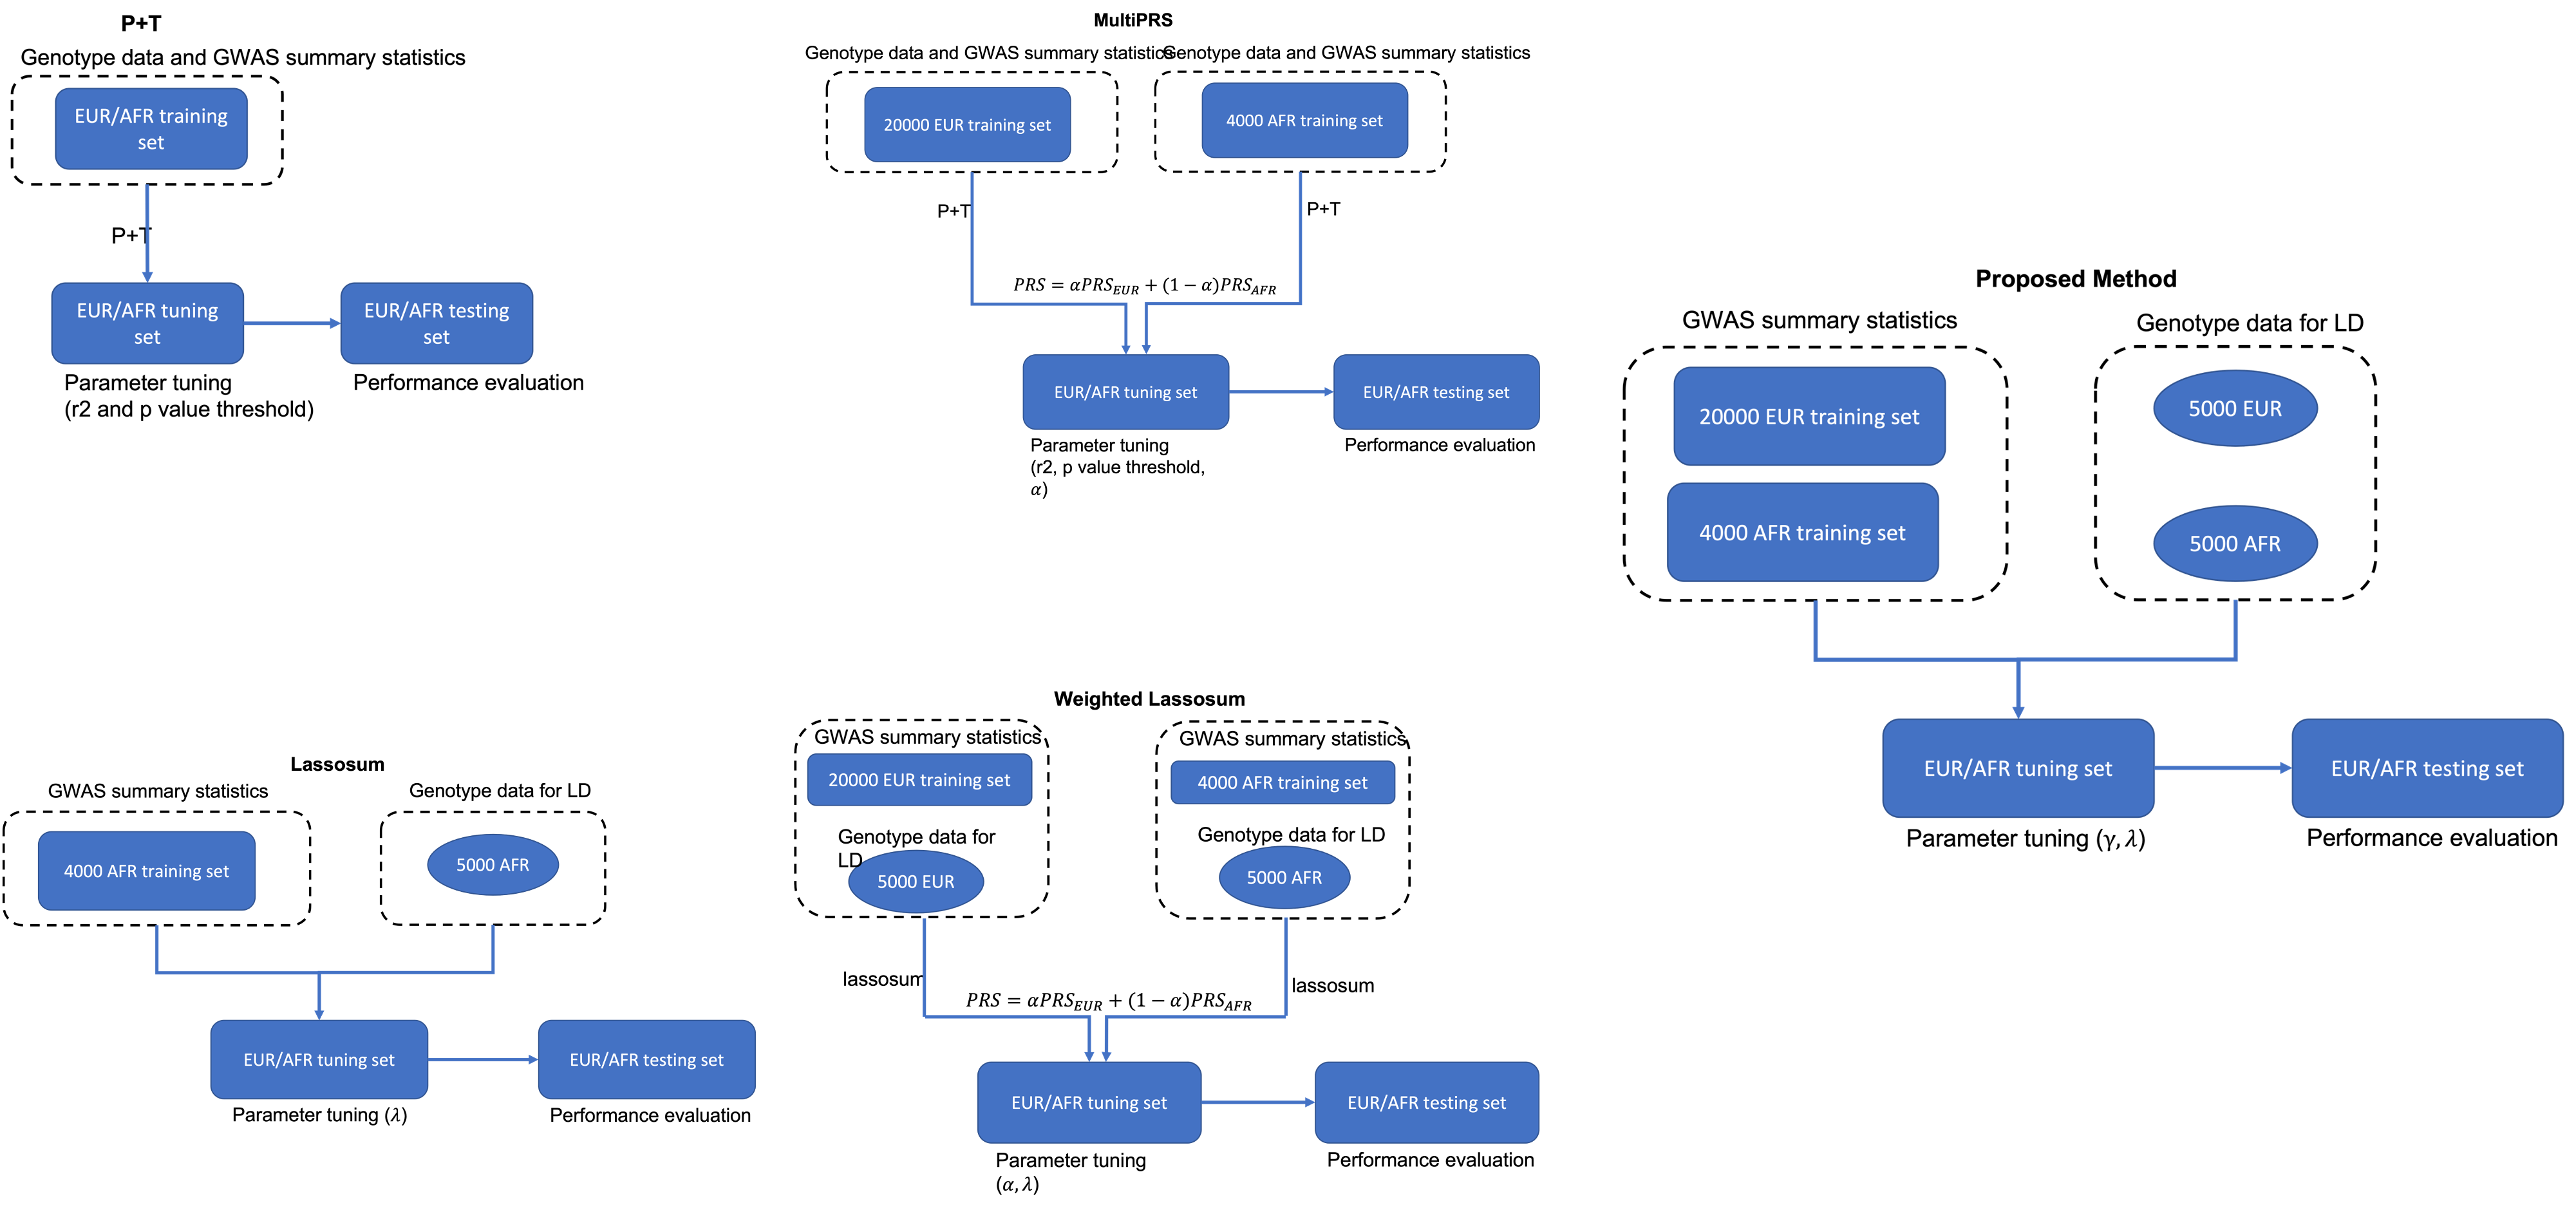
\includegraphics[scale=0.4]{images/Combined.png}}
      %\caption{gamma vs AUC}
   \label{fig:methods comparison}
\end{figure}

\end{frame}

\end{document} 